
% v2-acmsmall-sample.tex, dated March 6 2012
% This is a sample file for ACM small trim journals
%
% Compilation using 'acmsmall.cls' - version 1.3 (March 2012), Aptara Inc.
% (c) 2010 Association for Computing Machinery (ACM)
%
% Questions/Suggestions/Feedback should be addressed to => "acmtexsupport@aptaracorp.com".
% Users can also go through the FAQs available on the journal's submission webpage.
%
% Steps to compile: latex, bibtex, latex latex
%
% For tracking purposes => this is v1.3 - March 2012

\documentclass[prodmode,acmtkdd]{acmsmall} % Aptara syntax

% Package to generate and customize Algorithm as per ACM style
\usepackage[ruled]{algorithm2e}
\renewcommand{\algorithmcfname}{ALGORITHM}
\SetAlFnt{\small}
\SetAlCapFnt{\small}
\SetAlCapNameFnt{\small}
\SetAlCapHSkip{0pt}
\IncMargin{-\parindent}



% Our custom packages
\usepackage{times}
\usepackage{helvet}
\usepackage{courier}
\frenchspacing

\usepackage{url}
\usepackage{varioref}

% Small sections of multiple columns
\usepackage{multicol}
% Provides paragraphs of dummy text
\usepackage{lipsum}

\usepackage[super]{nth}

%\usepackage{subfig}
\usepackage{multirow}

\usepackage{amsmath, mathrsfs}
\usepackage{array} % to manage equations
\usepackage{amssymb}

%\usepackage{amsthm} %theorem like environments 
%\theoremstyle{plain} 		\newtheorem{thm}{Theorem}[section]
%\theoremstyle{definition} 	\newtheorem{defn}[thm]{Definition}
%\theoremstyle{remark}		\newtheorem{rem}{Remark}
%\newtheorem{lemma}[thm]{Lemma}

% in text graphics
\usepackage{tikz} 

% caption
\usepackage[font=small,format=plain,labelfont=bf,textfont=it]{caption}

% Set up the images/graphics package
\usepackage{graphicx}
\setkeys{Gin}{width=\linewidth,totalheight=\textheight,keepaspectratio}
\graphicspath{{figures/}}
% The following package makes prettier tables.  We're all about the bling!
\usepackage{booktabs}
% The units package provides nice, non-stacked fractions and better spacing
% for units.
\usepackage{units}

\usepackage{caption}
\captionsetup{compatibility=false}

\let\subcaption\undefined
\let\subfloat\undefined
\usepackage{subcaption}

% for side captions
\usepackage{sidecap}

%\newcommand{\argmax}{\operatornamewithlimits{argmax}}
\DeclareMathOperator*{\argmax}{arg\,max}



% Metadata Information
%\acmVolume{9}
%\acmNumber{4}
%\acmArticle{39}
%\acmYear{2010}
%\acmMonth{3}

% Document starts
\begin{document}

% Page heads
\markboth{K. Sarkar, H. Sundaram}{How Do We Find Early Adopters Who Will Guide a Resource Constrained Network Towards a Desired Distribution of Behaviors?}

% Title portion
\title{How Do We Find Early Adopters Who Will Guide a Resource Constrained Network Towards a Desired Distribution of Behaviors?}
\author{KAUSHIK SARKAR
\affil{Arizona State University}
HARI SUNDARAM
\affil{Arizona State University}}
% NOTE! Affiliations placed here should be for the institution where the
%       BULK of the research was done. If the author has gone to a new
%       institution, before publication, the (above) affiliation should NOT be changed.
%       The authors 'current' address may be given in the "Author's addresses:" block (below).
%       So for example, Mr. Abdelzaher, the bulk of the research was done at UIUC, and he is
%       currently affiliated with NASA.

\begin{abstract}
We identify influential early adopters that achieve a target behavior distribution for a resource constrained social network with multiple costly behaviors. This problem is important for applications ranging from collective behavior change to corporate viral marketing campaigns. In this paper, we propose a model of diffusion of multiple behaviors when individual participants have resource constraints. Individuals adopt the set of behaviors that maximize their utility subject to available resources. We show that the problem of influence maximization for multiple behaviors is NP-complete. Thus we propose different heuristics based on node degree, Influence Weight  and Immediate Adoption to select early adopters. We evaluate the effectiveness under three metrics: unique number of participants, total number of active behaviors and network resource utilization. We also propose heuristics to distribute the behaviors amongst the early adopters to achieve a target distribution in the population. We test our approach on synthetic and real-world topologies with excellent results. Our heuristics produce 15-51\% increase in resource utilization over the na\"ive approach.
\end{abstract}

\category{J.4}{Social and Behavioral Sciences}{}

\category{I.6.3}{Simulation and Modeling}{Applications}

\terms{Algorithms, Theory, Experimentation}

\keywords{Behavior diffusion, seed selection, social diffusion, social network, viral marketing}

\acmformat{Kaushik Sarkar, and Hari Sundaram, 2013. How Do We Find Early Adopters Who Will Guide a Resource Constrained Network Towards a Desired Distribution of Behaviors?}
% At a minimum you need to supply the author names, year and a title.
% IMPORTANT:
% Full first names whenever they are known, surname last, followed by a period.
% In the case of two authors, 'and' is placed between them.
% In the case of three or more authors, the serial comma is used, that is, all author names
% except the last one but including the penultimate author's name are followed by a comma,
% and then 'and' is placed before the final author's name.
% If only first and middle initials are known, then each initial
% is followed by a period and they are separated by a space.
% The remaining information (journal title, volume, article number, date, etc.) is 'auto-generated'.

\begin{bottomstuff}
%This work is supported by the National Science Foundation, under
%grant CNS-0435060, grant CCR-0325197 and grant EN-CS-0329609.

%Author's addresses: G. Zhou, Computer Science Department,
%College of William and Mary; Y. Wu  {and} J. A. Stankovic,
%Computer Science Department, University of Virginia; T. Yan,
%Eaton Innovation Center; T. He, Computer Science Department,
%University of Minnesota; C. Huang, Google; T. F. Abdelzaher,
%(Current address) NASA Ames Research Center, Moffett Field, California 94035.
\end{bottomstuff}

\maketitle

\section{Introduction}
This paper investigates how costly, multiple behaviors spread in social networks where individual have resource constraints. These constraints could include time, money or any material resource relevant to adopting the behavior.  The problem is challenging because the problem of finding early adopters or seeds is known to be computationally intractable. We develop heuristics to find early adopters that maximize multiple behavior adoption over resource constrained social networks.

Many of the pressing challenges facing contemporary society concern sustainability and public health. For example, how can sustainable behaviors---such as reducing individual energy consumption---be encouraged? How can participation in activities that reduce overall healthcare costs---such as compliance with preventive care routines and leading healthy lifestyles---be supported? These questions are termed as \textit{collective action} problems in the social sciences~\cite{Ostrom1999}. 

We are motivated by collective action problems to answer questions such as: how does a person's limited resources, including time, money or lack of tangible resources like a car or a bicycle, affect how she participates in real-world activities? A person interested in adopting a behavior (e.g. taking newspapers to a recycling station or voting) may fail to do so, due to
lack of resources.  A person may be interested in adopting multiple behaviors,
but each behavior has a cost. Current models of behavior adoption lack the idea that individuals may have significant resource constraints that preclude them from successfully adopting behaviors in which they are interested. Resource constraints not only limit individual participation, but also shape how behaviors spread in a network. We are interested in maximizing the use of resources available in a social network towards adopting a set of behaviors.

%Social network plays an important role in dissemination of information. People come to know about new ideas, information and habits through their friends, relatives and other social contacts. Often a person participates into a novel activity due to social influence. The phenomena of this person to person spread of new ideas, information or activities are often identified as social diffusion processes. When people adopt new behaviors due to the influence of other people in their social network the resulting diffusion process is called \textit{behavior diffusion} process. Adopting a new behavior like exercising or consuming organic products requires substantial commitment of resources on the part of the individual (as opposed to spreading a news article in twitter or Facebook). Consideration of this resource constraint at the individual level is important for behavior diffusion since presumable adoption of a new behavior would require long term commitment of some type from the person. For example, even if there is enough social influence, for a person to be able to adopt the habit of regular exercising, she should be able to make time to go to the gym. Moreover an individual's intrinsic interest in the activity plays a significant role in the adoption besides the social influence effect. A person must feel that regular exercising is beneficial for her long term well being to be motivated enough to adopt and continue the habit.

%Sometimes the social diffusion processes are so strong that new ideas or activities become quite popular within a short period of time. Something ''going viral'' colloquially refers to this sudden popularity. In the context of such social diffusion processes then it is naturally an interesting question to ask - how can we start such ''viral'' diffusion processes with some limitations on our resources? This is the core question of the seed selection problem. We are interested in addressing this question for behavior diffusion processes when multiple behaviors are diffusing at the same time. For multiple behavior diffusion processes on a social network of individuals with resource constraints the seed selection problem can be formulated to achieve a number of objectives. In this paper we are interested in the following objectives - maximizing the utilization of the individual resources in the social network, maximizing the spread of the behaviors, achieving a desired target distribution of behaviors in the social network.
%
%Although the seed selection problem has been studied extensively in the last decade (see Related Work), the context of those investigations were mostly propagation of a single influence. In contrast to that we are interested in a situation where multiple behaviors are diffusing at the same time and the individuals have constraints on the available resources for adoption. These assumptions are more realistic compared to the simpler theoretical models studied previously.
%
%Diffusion of behavior is an important process in the context of collective behavior change. The biggest problems of our age like global warming, depletion of non-renewable sources of energy etc. cannot be fought only through legislation at the government or international level. These problems require mass adoption of green, environment friendly practices like recycling, consuming locally grown food, using alternative sources of energy etc. Apart from the traditional viral marketing applications, we aim to contribute to the problem of mass adoption of sustainable behaviors.

In this paper, we develop a model of multiple behavior diffusion that captures the complex dynamics of multiple behavior adoption in resource constrained networks. Our work is the first of its kind, to the best of our knowledge to study the influence of individual resource constraints on multiple, costly behavior adoption. In our model, behaviors have associated costs and utilities that are independent of the individual. Mindful of the work by ~\cite{Aral09} and ~\cite{shalizi11}, individuals in our model evaluate a utility function for each behavior that combines intrinsic interest and social signals.  An individual adopts a behavior when she receives a social signal of sufficient strength, the behavior is of high utility and when she has the resources to do so. We use three metrics: unique number of participants, number of behaviors in the network and expected resource utilization. Then, we identify two problems: which seeds to select, and what behaviors they need to adopt to maximize each of the three metrics.

We develop several heuristics to identify seeds that maximize the expected resource utilization in the network. These heuristics are necessary since we show that the problem of seed selection to maximize expected utilization is NP-complete. We also develop a heuristic to address a simple question: how do we distribute behaviors amongst the seeds to achieve a target behavior distribution? We test our approach on synthetic and real-world topologies with excellent results. We show that two heuristics that evaluate Influence Weight  and Immediate Adoption provide very good solutions to the seed selection problems. We show that setting the seed behavior distribution to be proportional to the target behavior distribution produces excellent results. Our heuristics produce 15-51\% increase in resource utilization over the na\"ive approach.

The rest of the paper is organized as follows. In the next section we review the relevant literature. In Section~\ref{sec:model} we formally define our behavior diffusion model. In Section~\ref{sec:seed-selection} we define the seed selection problem, present different heuristics and compare their performance. In Section~\ref{sec:dist} we discuss different behavior distribution strategies and present simulation results. In Section~\ref{sec:target-dist} discuss how to achieve a target distribution of behaviors in the network. In Section~\ref{sec:disc} we discuss open issues and extensions.  Finally,  we present our conclusions in Section~\ref{sec:conclusion}.

\section{Related Work}
The literature on social diffusion processes in vast. Diffusion of innovation was studied in \cite{rogers62}. Subsequent work on modeling such processes through epidemiological models was carried out by \cite{bass69} which became well known as the \textit{Bass Diffusion Model} in the management sciences community. Another approach of explaining such processes through threshold based models were made popular by \cite{granovetter83}. In recent years the study of diffusion modeling has seen substantial development. \cite{Watts02} presents a threshold based model of global cascades and analyzes why certain networks may appear to be ''robust'' yet turn out to be fragile against such cascades.

Works of \cite{Domingos02} and \cite{Kempe03} initiated the study of the computational problem of seed selection in the context of a ''viral'' social diffusion process. \cite{Kempe03} formalized the algorithmic problem for \textit{Independent Cascade} and \textit{Linear Threshold} models, proved the intractability results and provided a greedy approximation algorithm to the problem. However the approximation algorithm incurred a huge computational cost in practice. \cite{Leskovec07} came up with CELF technique to reduce the simulation cost of the algorithm. \cite{Chen09} tried to address that problem by coming up with computationally cheap heuristics that match the performance of the approximation algorithm. A complementary data mining perspective of inferring the diffusion model parameters from the past interactions the was taken by \cite{Saito08}, \cite{Goyal10} and \cite{Mathioudakis11}. 

Our work is informed by these literature, but is markedly different in a number of aspects. Much of the existing literature is concerned with diffusion of a single influence, while simultaneous diffusion of multiple influences is a more realistic scenario. Moreover none of these works take constraint on user resources into account and thereby does not apply directly to our problem of long term adoption of behaviors. \cite{Bharathi07} and \cite{Carnes07} discuss the problem of multiple competing influences, but they also do not incorporate the resource constraints or the utility maximizing behavior of social agents into their models. To the best of our knowledge the present work is the first investigation of the seed selection problem for multiple behavior diffusion in a resource constrained social network.

Next we mention a few interesting critiques of the study of social diffusion. The study of social diffusion and information contagion has met with its fair share of criticism. \cite{Aral09} argues that in their observational study more than $50\%$ of the perceived behavior contagion can be attributed to homophily instead of social influence. However \cite{shalizi11} have shown that homophily and social influence are generically confounded in social diffusion processes and it in general not easy to distinguish between the two effects. We have tried to take this observation into account while developing our model where. In our model the diffusion process is not exclusively driven by the social influence effects but an individual's intrinsic characteristics (i.e. resource constraint) also plays an important part in the adoption decision making.  An important critique of the study of modeling mass adoption through epidemic like contagion models is put forward by \cite{Goel12}. They have analyzed a number of real world product diffusion events and found out that in most of the cases the diffusion stops within one degree of the initial adopting seed, thus drawing a sharp contrast with multi-step person to person contagion of influence. It is however unclear if their findings will generalize to collective action problems, where participating individuals express interest in adopting a behavior (e.g. eating healthy foods, take a flu shot). As we discuss in our open issues section (Section~\ref{sec:disc}), there may be confounding effects between the communication problem and the decision making problem. That is, behavioral diffusion can halt in the presence of poor communication.

\section{Models of Behavior Adoption under Resource Constraint}\label{sec:model}
In this section we introduce our behavior diffusion models. First we will describe our model of multiple behavior diffusion in a resource constrained network in the most general form. Next we will present a simplified version of the general model which will provide us with some analytical insight into the algorithmic problems to be defined in the next section. Then we will introduce metrics, including resource utilization, unique participation and number of behavior adoptions to evaluate the behavior adoption process.

\subsection{A Model of Multiple Behavior Diffusion in a Resource Constrained Social Network} \label{sub-sec:model}
We now describe the model for each user, the properties of each behavior and the behavior adoption process. Conceptually our behavior adoption model can be described as follows - an individual adopts a new behaviors if the behavior has some value to him, or he has some interest in the behavior (intent), many of her friends have adopted the behavior (social signal), and she has enough available resource to pursue it (resource). Her payoff from adopting that behavior will be determined by her intent and social signal. Figure \ref{fig:concept-1} and \ref{fig:snap-concept-1} shows the idea in a simple way. Next we try to describe this idea formally.

\begin{figure}[htb]
\begin{centering}
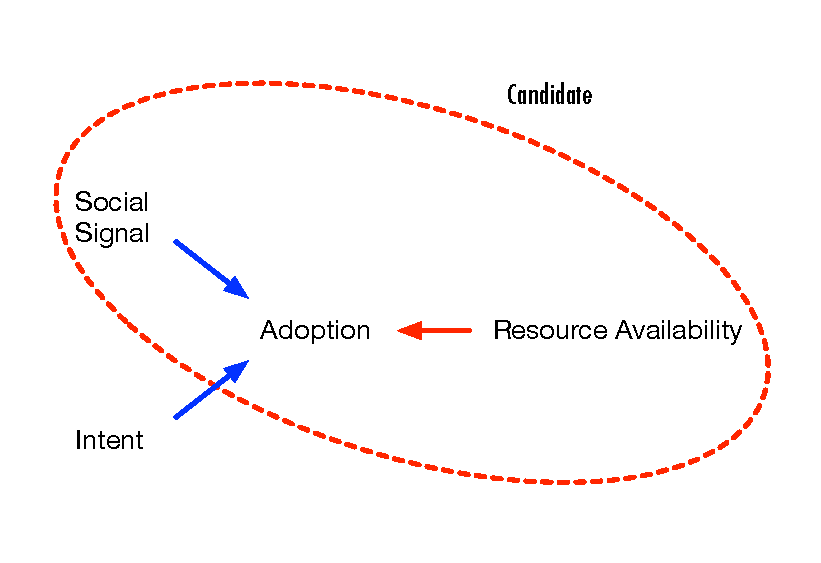
\includegraphics[width=\columnwidth]{figs/candidate}
\par\end{centering}
\caption{Sufficient social signal, intent and resource make an individual a candidate for adoption of a behavior.}\label{fig:concept-1}
\end{figure}

\begin{figure}[htb]
\begin{centering}
\includegraphics[width=\columnwidth]{"figs/candidate and payoff"}
\par\end{centering}
\caption{Payoff for adopting a behavior comes from an individual's intent and social signal.}\label{fig:concept-2}
\end{figure}

We represent the social network with an undirected graph $G=(V,E)$. Each node $v \in V$ of the graph $G$ represents an individual and an edge $e \in E$ between two nodes indicate a social relationship between the two individuals. 

We wish to spread $k$ behaviors in the social network. Each behavior $i$ has an associated cost $c^i$ and a utility $u^i$. The cost refers to the cost of adoption and the utility refers to the intrinsic utility gained by an individual by adopting this behavior. In a simplification, we assume that both the cost $c^i$ and the utility $u^i$ of behavior $i$ are intrinsic to the behavior and independent of the individual who adopts the behavior. Without loss of generality, we assume that $0 \leq c^i, u^i \leq 1$.

Individuals are resource constrained: an individual may have limited time, money or may not possess other material resources to adopt a behavior. Therefore, we assign a \textit{fixed} resource $r(v)$ for each individual $v \in V$ towards adopting behaviors. The resource satisfies $0 \leq r(v) \leq 1$. For example, if we assume that individuals' resources are independent and identically distributed then the resource value $r(v)$ can be assumed to be obtained from a uniformly distributed random variable $U(0,1)$.  Let $N(v)$ denote the set of neighbors of $v$ in the network. Then we assume that a neighboring node $u$ asserts a social influence on node $v$ with weight $1/|N(v)|$.  

An individual will adopt a behavior $i$ when she receives a strong social signal, has the resources to do so and when the behavior is of a sufficiently high utility.  An individual $v$ adopts a behavior $i$ when the social signal exceeds a threshold $\theta^i(v)$, where $0 \leq \theta^i(v) \leq 1$. We assume that each individual $v$ has a different, fixed, threshold for each behavior, and that each threshold is obtained from a uniformly distributed random variable $U(0,1)$.  An individual $v$ can adopt a behavior $i$ provided the cost $c^i$ is less than $r(v)$, the available resources. The payoff $p^i(v)$ for a behavior $i$ is defined as the weighted sum of the intrinsic utility $u^i$ and the local network utility $l^i(v)$. That is, $p^i(v) = wu^i + (1 - w)l^i(v)$. Where, $w$ denotes the relative weight of the intrinsic utility and where $l^i(v)$ denotes the sum of influence weights---the social signal---exerted on $v$ by its neighbors who have adopted behavior $i$. If there are multiple behaviors that can be adopted, an individual will adopt a subset that maximizes payoff. 

Let us examine the diffusion of behavior over time, to illuminate the key ideas. The process takes place over discrete epochs\footnote{Notice that while actions in a network are asynchronous, we can choose an appropriate time granularity for analysis to assume synchronized decision making.}. We assume each node is aware of the behaviors adopted by her neighbors. The individual $v$ first identifies all candidate behaviors. A behavior $j$ is a candidate to be adopted if two conditions hold. First the social signal strength for behavior $j$ must exceed the threshold for that behavior at node $v$---$l^j(v) \ge \theta^j(v)$. Second, the individual $v$ must have the resources to adopt the behavior---$r(v) \ge c^j$.  The first condition is the familiar Linear Threshold (LT) model \cite{Kempe03}. Since there are multiple behaviors, the individual $v$ chooses a set of behaviors that will maximize the total payoff (i.e. the sum of payoffs $\sum_i p^i(v)$ over candidate behaviors) subject to the condition that the sum of the adoption costs of the behaviors are less than the resource constraint. That is $\sum_i c^i \leq r(v)$. At every epoch, the individual $v$ evaluates all behaviors, including behaviors already adopted, to evaluate payoff. %In a variation of the model, we can introduce \textit{inertia} into the system, by increasing the intrinsic utility of adoption by a fixed constant. 
The behavior diffusion process continues until no additional adoption is possible. 

In our diffusion model, we assume that the total resources available $r(v)$ at each node  are known, while the threshold for adoption $\theta$ for any behavior is unknown. This assumption is reasonable if when people are willing to make public their available resources to participate in a set of behaviors. This can arise say in a private, mobile social network app focused on adoption of healthy behaviors including wellness, healthy eating and exercise, where individuals join the network to participate in healthy behaviors but each individual is resource limited. An individual may declare that she has only one hour to spend on exercise each week, but would like to be nudged to participate in a health-related activity.

Figure \ref{fig:model} shows an illustration of the dynamics with a four node network where three different behaviors - (1) recycling, (2) using public transport and (3) eating organic food are spreading. At time step $t$ the state of the network is shown in \ref{fig:state-before}. At this time step, for $v$, the social signal of eating organic food is weak. So $v$ considers only recycling and using public transport. After maximizing payoff subject to the resource constraint, $v$ adopts only recycling. Although public transport has strong social signal, $v$ cannot adopt that behavior because it does not have enough resource. Notice that the payoff for recycling is higher than that of public transport, though the intrinsic utility of recycling was lower than that of public transport. 

%viewport=1.25in 5in 6in 10.75in
%viewport=1.75in 4.5in 7in 11in

\begin{figure}[h]
	\parbox{.4\linewidth}{
	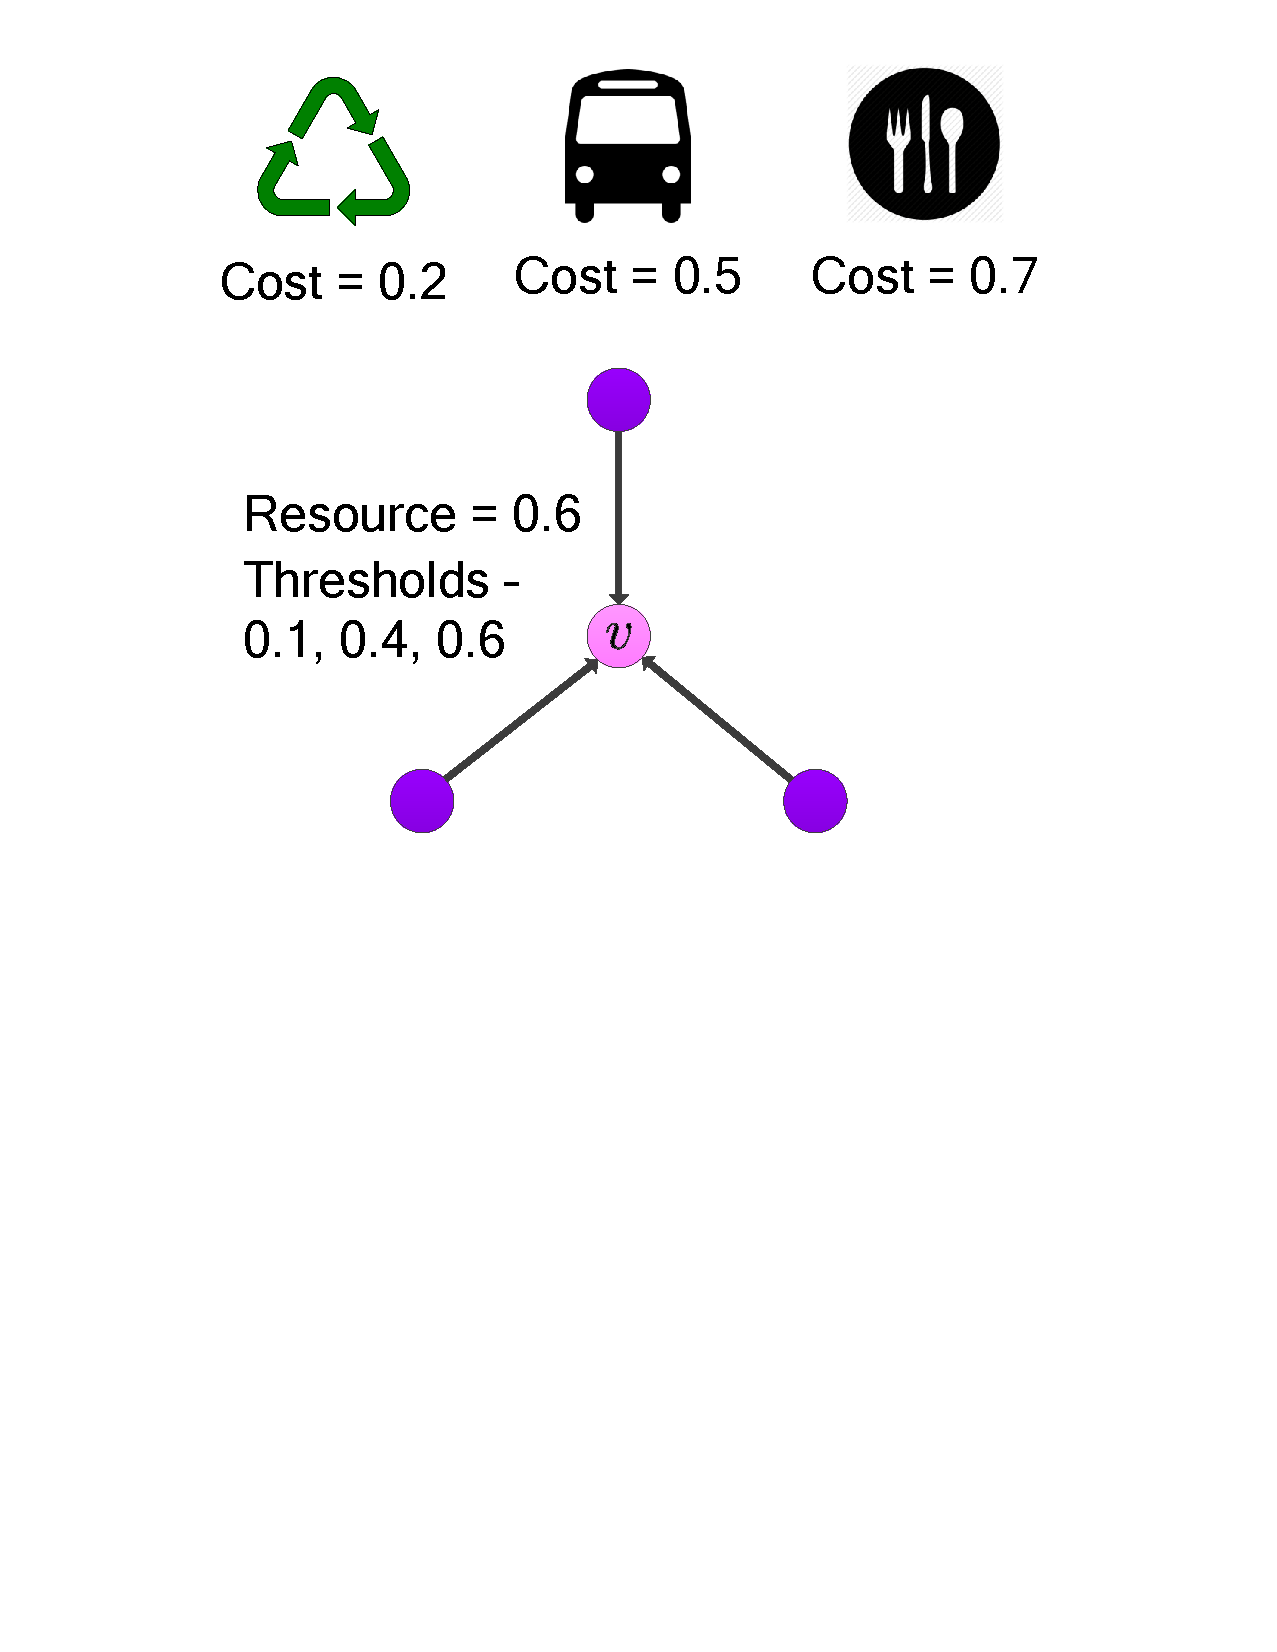
\includegraphics[trim=50 400 125 10, width=\linewidth]{figs/timeline-1a}}%
	\hspace{.2\linewidth}%
	\parbox[][][t]{.4\linewidth}{%
	\subcaption{The three beahviors - (1) recycling, (2) using public transport, and (3) eating organic food with respective costs as well as the network is shown. The intrinsic utility of the behaviors are same as the cost. So $c^1=u^1=0.2, ~c^2=u^2=0.5, ~c^3=u^3=0.7$. Resource of the node $v$, $r(v)=0.6$, and the thresholds are - $\theta^1(v)=0.1,~\theta^2(v)=0.4,~\theta^3=0.6$.}}
	\parbox{.4\linewidth}{
	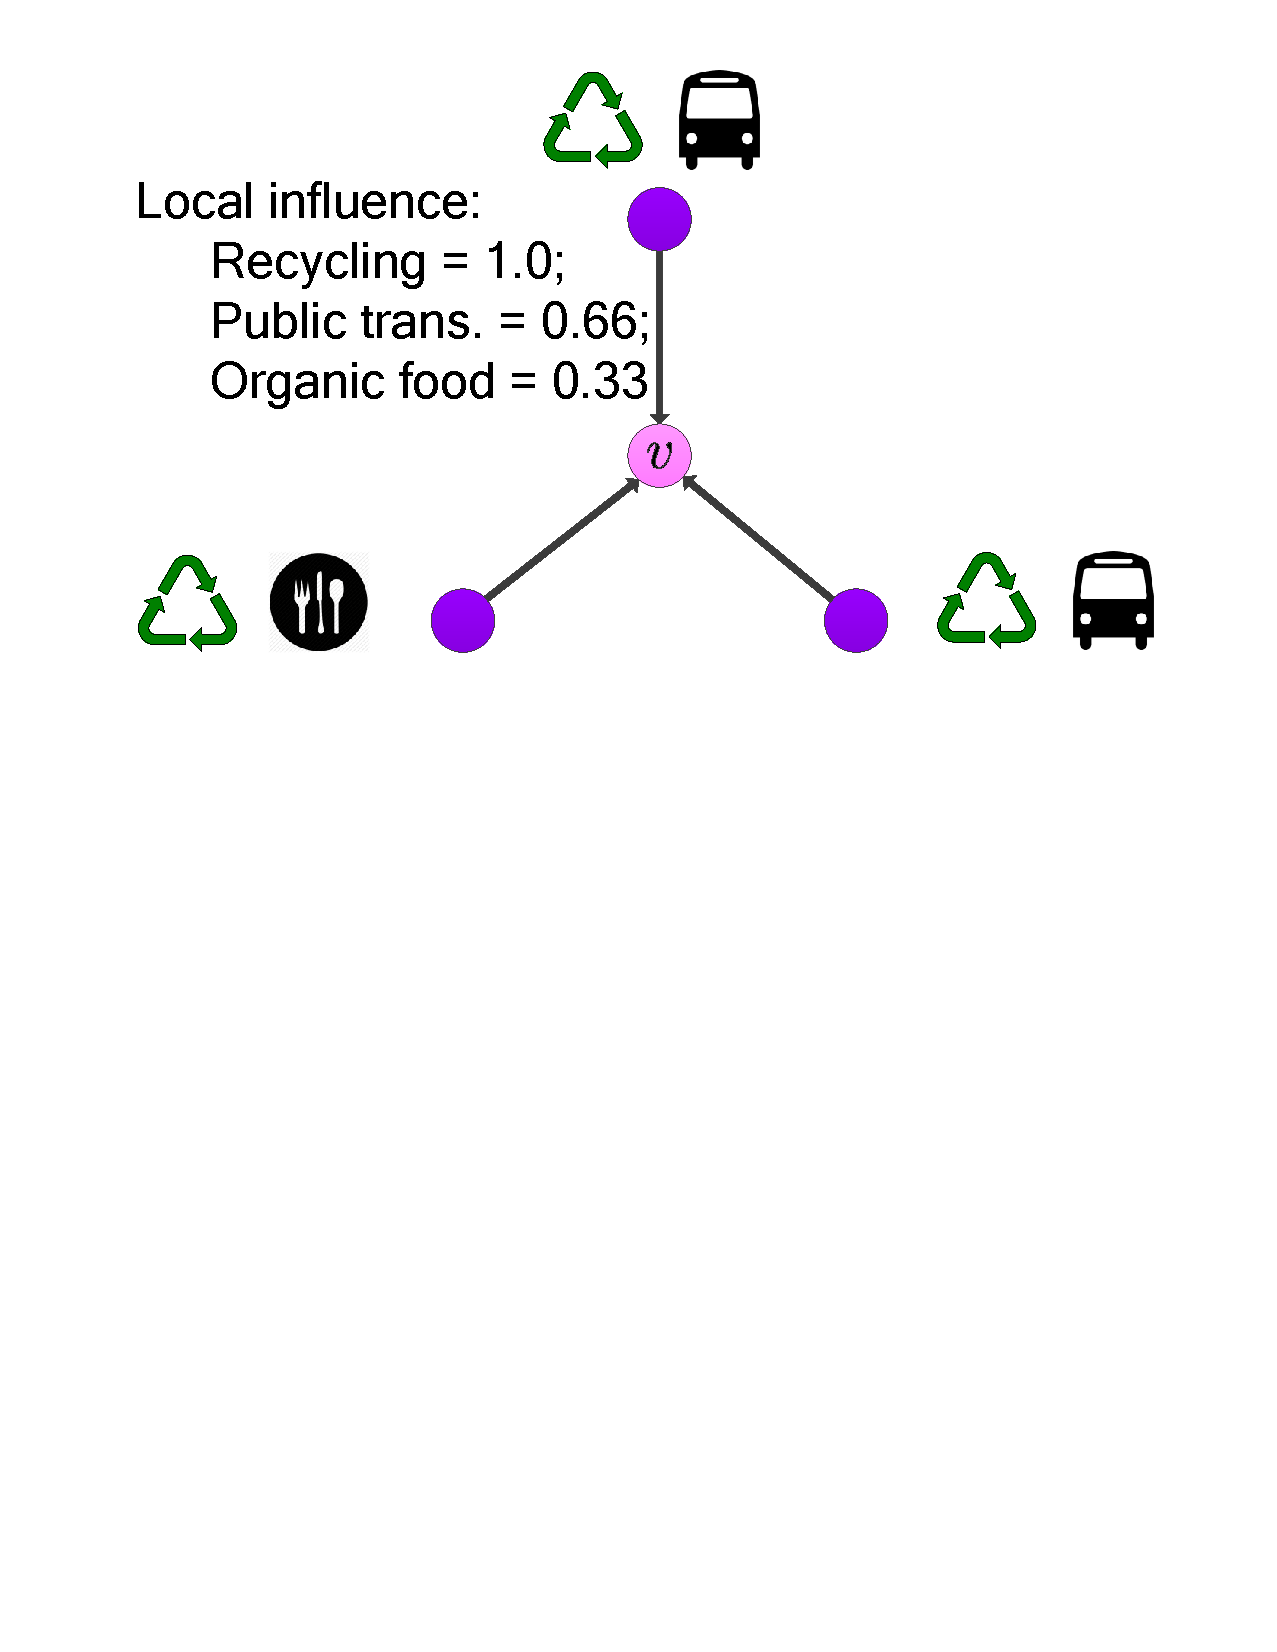
\includegraphics[trim=85 450 125 0, width=\linewidth]{figs/timeline-2a}}%
	\hspace{.2\linewidth}%
	\parbox[][][t]{.4\linewidth}{%
	\subcaption{This is the network at some time step $t$. All three of the neighbors of $v$ have adopted recycling, two of them have adopted public transport, and only one of them is eating organic food. $v$ has not adopted any behavior yet. The local influences for the three behaviors are as follows - $l^1(v)=1.0,~l^2(v)=0.66,~l^3(v)=0.33$.}\label{fig:state-before}}
	\parbox{.4\linewidth}{
	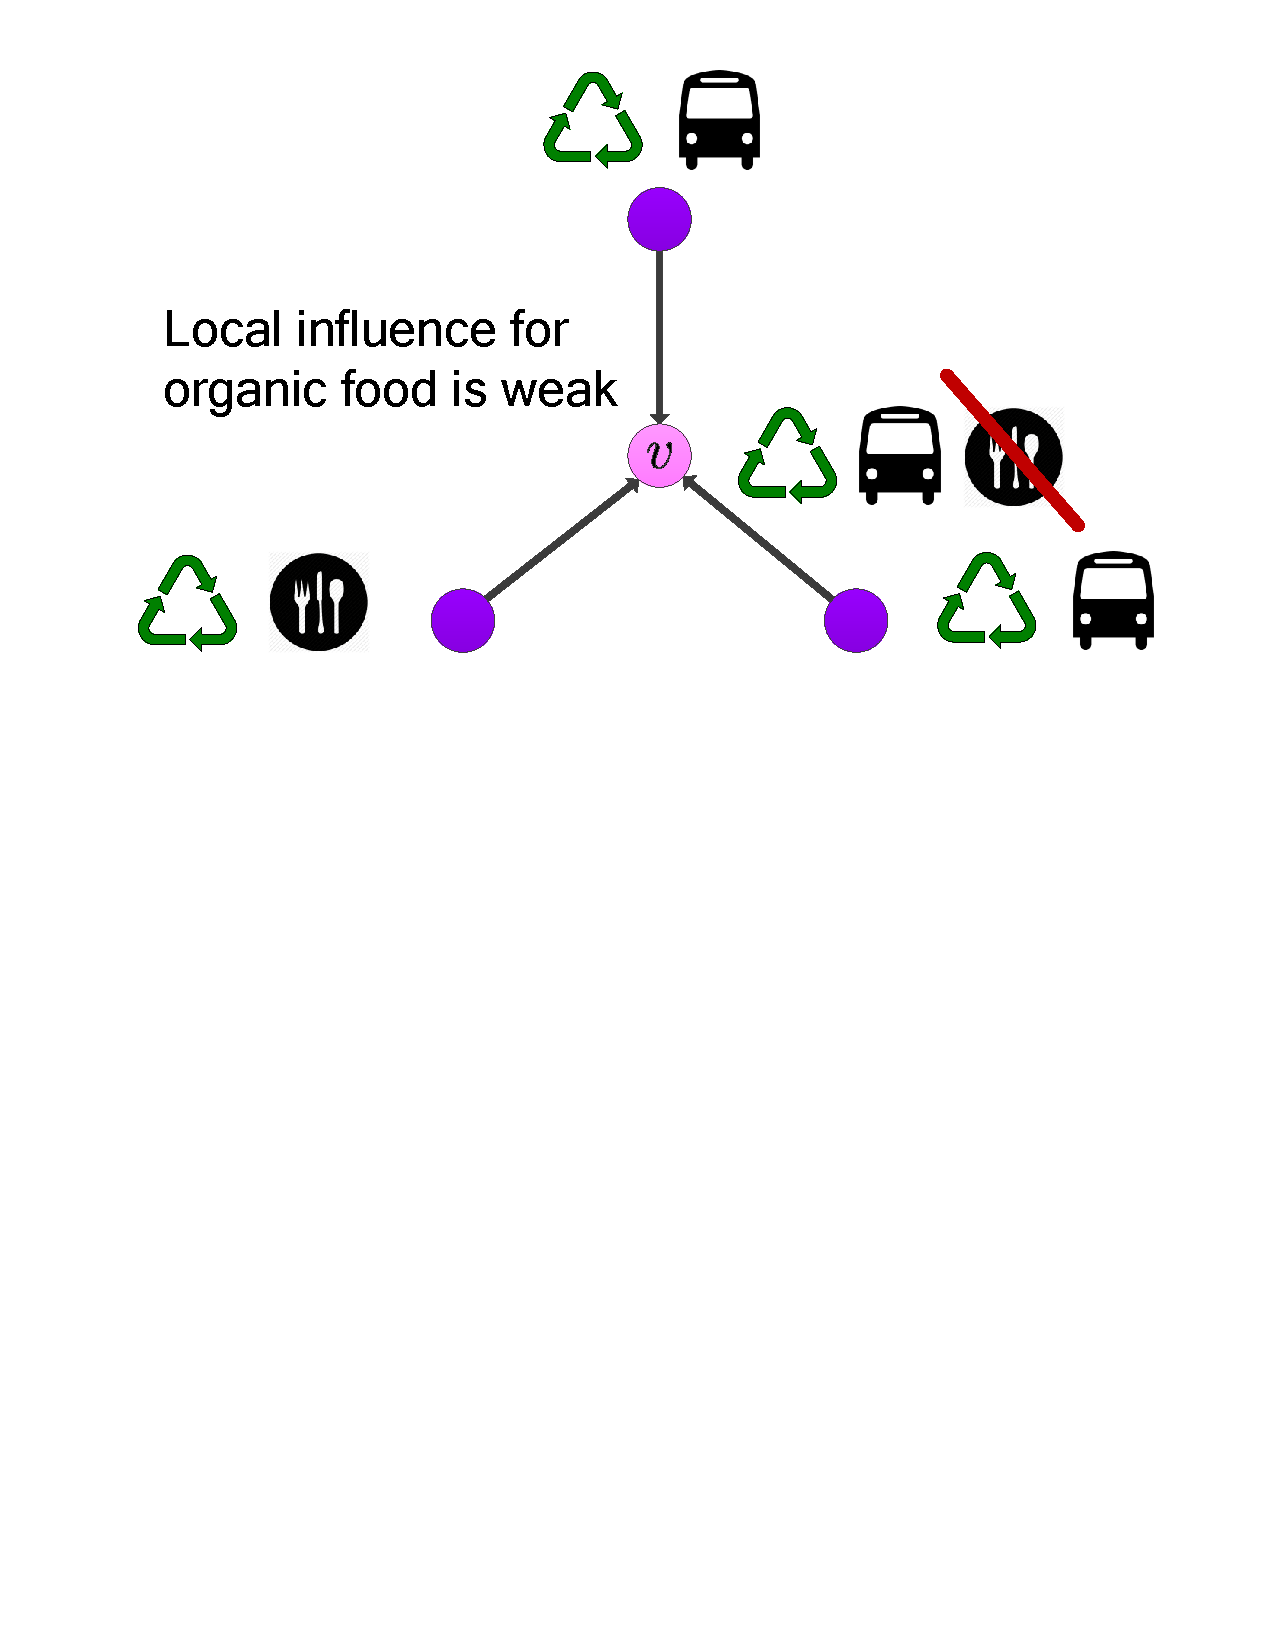
\includegraphics[trim=85 450 125 30, width=\linewidth]{figs/timeline-3a}}%
	\hspace{.2\linewidth}%
	\parbox[][][t]{.4\linewidth}{%
	\subcaption{Local influence for organic food is less than the threshold, i.e $l^3(v)<\theta^3(v)$. So $v$ will not consider organic food for adoption.}}
	\parbox{.4\linewidth}{
	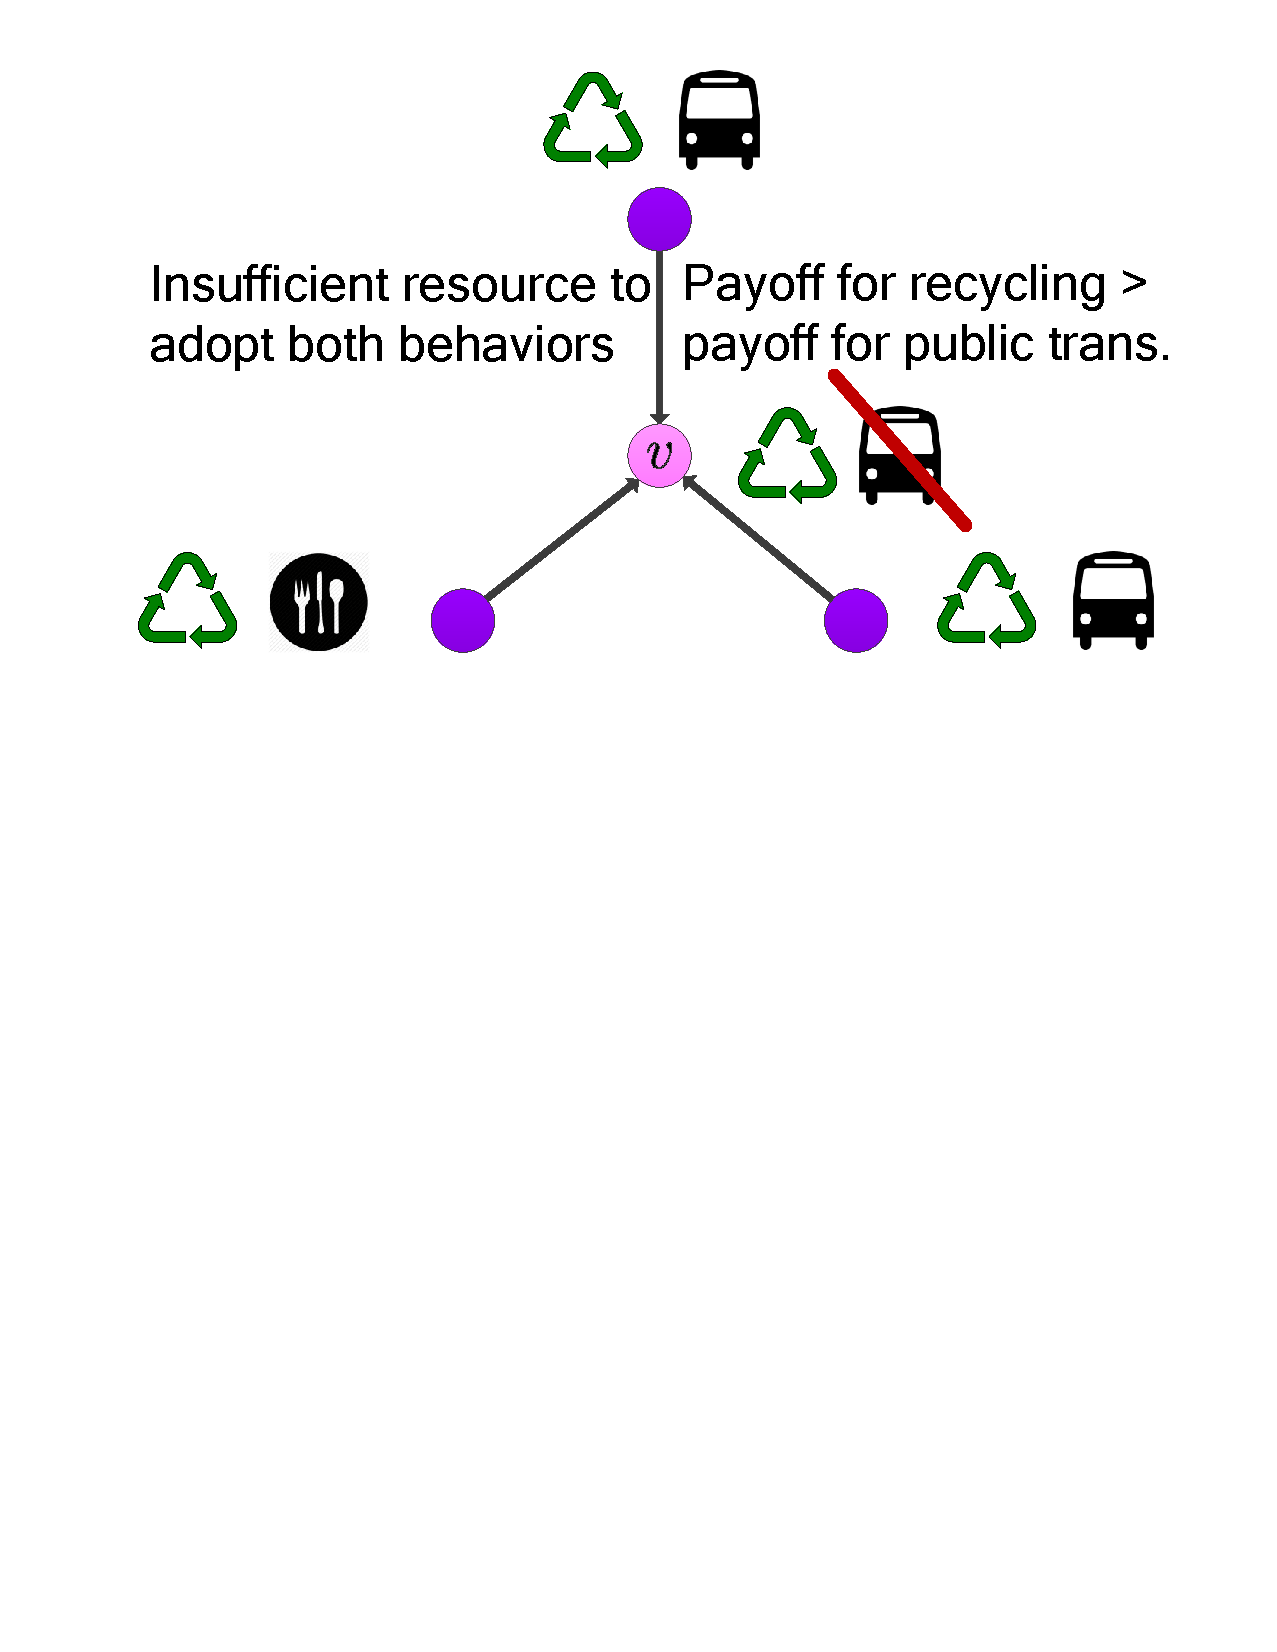
\includegraphics[trim=85 450 125 30, width=\linewidth]{figs/timeline-4a}}%
	\hspace{.2\linewidth}%
	\parbox[][][t]{.4\linewidth}{%
	\subcaption{$c^1+c^2>r(v)$, so $v$'s resource is insufficient for adopting both recycling and public transport. Payoff for recycling, $p^1(v)=0.6$, and payoff for public transport, $p^2(v)=0.58$. For $v$ the payoff for recycling is higher than the payoff for using public transport though the intrinsic utility of public transport is higher than that of recycling. So $v$ will adopt recycling at the end of time step $t$. }}
	\caption{Multiple behavior adoption model.}\label{fig:model}
\end{figure}


%\subsection{A Simplified Sticky Model} \label{sub-sec:simple-model}
%In this section we present a simplified version of the multiple behavior diffusion model defined in the previous section. 
Next we present a simplified version of the aforementioned multiple behavior diffusion model. Although the previous model makes fewer assumptions and is a more faithful representation of reality, it is cumbersome to deal with analytically. The simplified model, which we will call the "Sticky" model, makes stricter assumptions and affords us some interesting analytical insights on the fundamental processes of the multiple behavior diffusion phenomena.

The difference between the simplified model and the original model is in the temporal unfolding of the diffusion process. Unlike the original model, in the simplified model once a node adopts a behavior at some time step, it does not get rid of that behavior in the subsequent time steps. The behavior adoption is \textit{progressive} \cite{Kempe03}. So once a behavior is adopted by a node, it "sticks" with that node (hence the name \textit{Sticky} model). At each time step each node selects the candidate behaviors for adoption from only those behaviors that are not already adopted by that node. Otherwise the selection criteria are the same as the original model. The node then adopts the set of candidate behaviors that maximize his payoff subject to the constraint that the combined cost of the newly adopted behaviors is less than the remaining resource of the node. 

%Another difference is that in this model nodes do not consider local network utility $l^i(v)$ while calculating their payoffs. The payoff of a node from adopting a behavior is simply the intrinsic utility of that behavior. All the other properties of the nodes and the behaviors in the Sticky model are the same as in the original model.

\subsection{Measurement of the Diffusion}
We measure the effectiveness of the diffusion process with three metrics: total participation, total adoption and resource utilization. Since the behavior adoption is a stochastic process, we compute the expected value of each metric through simulation.

\subsubsection{Total Participation}
This metric counts the the expected number of individuals who have adopted at least one behavior (i.e. become active) during the process. One goal for an advertiser who is interested in behavior adoption may be to maximize the total number of unique adoptees. Exact computation of this metric is an intractable problem (\#P-hard - \cite{Chen10}). 

\subsubsection{Total Adoption}
In contrast to total participation, we need to keep track of the total number adoptions of any behavior during the diffusion process. This metric counts the expected number of adoptions over all the behaviors. Notice that since an individual can adopt more than one behavior, total adoption cannot be less than total participation. For the familiar single behavior adoption problem, these two metrics will have same value.

\subsubsection{Resource Utilization}
This metric captures the \textit{efficiency} of the network to adopt costly behaviors. 
Not all resources available in a social network may be used for behavior adoption. This is  because individuals have variable resources, and they may be unable to adopt the subset of behaviors that fully takes advantage of their desire to participate because of two reasons. First, they may have many more resources than needed to adopt a behavior. Second, if their friends have limited resources, then the social signals that they receive will be about adopting low-cost resources, and hence a particular individual may never see costly behaviors in their social circle that they could potentially adopt.  let us assume that a node $v$ with resource $r(v)$ has adopted one or more behaviors. At the end of the diffusion process this individual has adopted a set of behaviors with total cost of adoption $s$, where  $s \le r(v)$. Therefore the individual has $r(v)-s$ amount of his resource remaining unused. \textit{Resource utilization} is the expected ratio of total utilized resource to the total amount of available resource of all the individuals in the social network. 

\section{The Seed Selection Problem} \label{sec:seed-selection}
In this section we introduce the first algorithmic problem that we want to address in the context of multiple behavior diffusion in a resource constrained social network. This problem is called \textit{seed selection} problem. In the next section we will formally define this problem. Then we will describe and analyze different strategies for solving the problem. Then we will provide experimental evaluation of those strategies on synthetic as well as real world social networks.

\subsection{Problem Definition}
There are two key problems: we need to identify the set of early adopters or seed nodes and we need to determine which behaviors ought to be adopted by each seed node. We assume that the number of initial adopters is small in comparison to the size of the network. This is reasonable as it corresponds to an advertiser with a finite budget to persuade the seeds to adopt. Here we identify two subproblems which are related to seed identification. To simplify things, in this section we will assume that the behaviors are uniformly distributed over the seed set.

Next, we identify four subproblems; the first two refer to seed identification while the last two are concerned with behavior distribution in the seeds.

\subsubsection{P1: Resource Utilization Maximization:} Given a fixed seed budget $b$ and a fixed distribution of behaviors in the seed set, we want to select $b$ nodes in the network such that the resource utilization metric is maximized.

\subsubsection{P2: Total Participation (or Adoption) Maximization:} Given a fixed seed budget $b$ and a fixed distribution of behaviors in the seed set, we are interested in finding $b$ nodes in the network that maximize the total participation (or total adoption) in the network.

\subsection{Which Nodes Do We Pick?} \label{sub-sec:heuristics}
In this section we develop algorithms and heuristics to pick seed nodes to address the seed selection problems. First we show that the seed selection problem is NP-complete. Next we show that it is possible to construct an approximation algorithm with good approximation guarantee for the seed selection problem for the Sticky model. Then, we will develop heuristics based on node degree, Influence Weight  and Immediate Adoption for the general behavior diffusion model under resource constraint.

\subsection{NP-Completeness}\label{sec:NP}
It can be easily shown that the optimization problems P1 and P2 are NP-complete. We show that influence maximization problem for LT model, which is proven to be an NP-complete problem \cite{Kempe03}, is a special case of P1. Let the number of behaviors $k=1$ and the cost of adoption of that behavior is also $1$. Each node $v$ is allocated resource $r(v)=1$. For these values of the parameters our multiple behavior diffusion model reduces to the LT model of influence propagation and resource utilization can be calculated as the ratio of the spread and total number of nodes in the network. So maximizing the resource utilization translates into maximizing the spread. Same transformation applies to problem P2 also since total participation (and total adoption) is identical to the spread in the one behavior case. Next, we propose a number of heuristics to solve the problem.

\subsection{Approximation Algorithm for the Sticky Model} \label{sub-sec:approx-algo}
In this section we will provide an approximation algorithm for the problem P2 (total participation maximization) under the simplified Sticky model of multiple behavior diffusion. Note that all the three problems - P1, P2 and P3 are still NP-hard in the Sticky model. We will achieve our goal by first showing that the total participation function satisfies a property called submodularity which will lead us to the construction of a standard approximation algorithm for the problem.

\subsubsection{Submodularity of Total Participation}
In this section we will show that the total participation function for the sticky model is submodular. Throughout this section we will assume that the $k$ behaviors are indexed in the ascending sorted order of their cost. For a given set $S$ of seeds for the $k$ behaviors, let $\sigma(S)$ denote the \emph{total participation} i.e. the expected number of active nodes at the end of the process. We will show that $\sigma(S)$ is a submodular function. 

\begin{theorem}
    For an arbitrary instance of the Sticky Multiple Behavior Diffusion model the total participation function $\sigma(.)$ is submodular.
\end{theorem}

\begin{proof}
    The proof consists of two steps - first we define an equivalent alternative process of the Sticky Multiple Behavior Diffusion process and then we prove the submodularity for the equivalent process.
    
    \emph{Alternative process:} For the alternative model we would like to distinguish between the behaviors a node can adopt and those that it cannot under any circumstances. If the cost of adoption of a behavior is greater than the available resource of a node then that node can never adopt that behavior. Since the behaviors are indexed in the ascending sorted order of their cost, this distinction can be made by a single indicator variable. For each node $v$, let us define $\kappa(v)$ as the largest index $j$ such that $c^j\le r(v)$. If $v$ does not have enough resource to adopt any of the behaviors then $\kappa(v):=0$. At the beginning of the process each node $v$ selects at most $\kappa(v)$ edges by repeating the following random edge selection process $\kappa(v)$ times - $v$ selects the edge $vw$ with probability $b_{v,w}$ and no edge with probability $1-\sum_{w \in N(v)}b_{v,w}$, where $b_{v,w}$ denotes the influence weight exerted by the neighbor $w$ on $v$ and $\sum_{w \in N(v)}b_{v,w} \le 1$; if an edge is selected then that edge is designated as the \emph{live} edge for the behavior $i$. All the other edges are considered \emph{blocked} for that behavior. So $v$ selects at most one edge for each of the $\kappa(v)$ behaviors. In this model we start with $k$ sets of seeds for each of the $k$ behaviors. In time step $t$, a node considers behavior $i$ for adoption if the behavior is not already adopted by it and it is reachable via its live edge designated for that behavior from a node which has already adopted behavior $i$ in time step $t-1$. The node then adopts a subset of all considered behaviors that maximizes its total payoff subject to the constraint that the combined cost is less than the remaining resource. Once a node adopts a behavior it becomes \textit{active}. This model is also sticky in nature. When a node adopts a behavior it never gets rid of it. We will show that this process is stochastically equivalent to the Sticky Multiple Behavior Diffusion model described before.
    
    \begin{lemma}
            For a given seed set $S$, the following two distributions over the set of nodes are the same:
            \begin{enumerate}
                \item The distribution over active sets obtained by running the Sticky Multiple Behavior Diffusion model to completion starting with $S$. 
                \item The distribution over sets of active nodes reachable from $S$ via live edges under the random selection of edge model described above.
            \end{enumerate}
    \end{lemma}
    
    First we provide the proof for the simpler case when $k=1$, i.e. there is only one behavior. This case is very similar to the Linear Threshold (LT) model described in \cite{Kempe03}. We only need to consider the nodes $v$ with $r(v)\ge c^1$. If we delete all the nodes with $r(v)<c^1$ (and the associated edges) then our model degenerates to the LT model. Here we repeat that proof. We argue by induction over the time step $t$. Let $S_t$ be the set of nodes who have adopted behavior $1$ at the end of time step $t$ for the Sticky Multiple Behavior Diffusion Model with $k=1$. We need to know the probability that a node $v$ with $r(v)\ge c^1$ that have not yet adopted behavior $1$ at the end of time step $t$ will adopt the behavior in the next time step $t+1$. This probability is the same as the probability that the nodes in $S_t\setminus S_{t-1}$ will push the influence weight of $v$ over its threshold, given that the threshold was not already crossed. This probability is given by $\frac{\sum_{w\in S_{t}\setminus S_{t-1}}b_{v,w}}{1-\sum_{w\in S_{t-1}}b_{v,w}}$. 
    
    For the alternative random model each node $v$ with $r(v)\ge c^1$ selects at most one live edge randomly at the beginning of the process. Under this model we need to compute the probability that a node $v$ with $r(v) \ge c^1$ that has not adopted behavior $1$ at the end of time step $t$ will adopt it in the next time step. This probability is precisely same as the probability that the live edge of $v$ comes from one of the nodes in $S_t\setminus S_{t-1}$, given that it did not came from $S_{t-1}$. This probability is also given by $\frac{\sum_{w\in S_{t}\setminus S_{t-1}}b_{v,w}}{1-\sum_{w\in S_{t-1}}b_{v,w}}$. So by induction we find that the two processes define the same distribution over the active sets. Next we provide the proof for the general case.
    
    \begin{proof}
        We prove the claim by induction on the time step $t$. Clearly the claim is true for $t=0$. We define $S_{t}^{i}$ as the set of active nodes with behavior $i$ at the end of time step $t$ of the Sticky
        Multiple Behavior Diffusion model. Let $S_{t}:=\cup_{i=1}^{k}S_{t}^{i}$. Notice that $S_0=S$. Suppose a node $v$ is not active at the end of time step $t$ and $\kappa(v)=\kappa \ne0$. Then the probability that $v$ will become active at the end of time step $t+1$ is equal to the probability that the nodes in $S_{t}\setminus S_{t-1}$ will push the influence weight of at least one of the first $\kappa$ behaviors over its corresponding threshold value, given that none of those thresholds were already crossed. This probability is 
        
        \[
        1-\prod_{i=1}^{\kappa}\left(1-\frac{\sum_{w\in S_{t}^{i}\setminus S_{t-1}^{i}}b_{v,w}}{1-\sum_{w\in S_{t-1}^{i}}b_{v,w}}\right)
        \]
        
        
        On the other hand we run the live edge reachability process as described above and denote by $S_{t}^{i}$ the set of all nodes with behavior $i$ at the end of time step $t$. Let $S_{t}:=\cup_{i=1}^{k}S_{t}^{i}$. If node $v$ is not active at the end of time step $t$ with $\kappa(v)=\kappa \ne 0$, then the probability that it will be active at the end of time step $t+1$ is equal to the probability that at least one of its $\kappa$ live edges comes from the nodes of $S_{t}\setminus S_{t-1}$ (with the corresponding behavior), given that none of those live edges came from $S_{t-1}$. This probability is also given by - 
        
        \[
        1-\prod_{i=1}^{\kappa}\left(1-\frac{\sum_{w\in S_{t}^{i}\setminus S_{t-1}^{i}}b_{v,w}}{1-\sum_{w\in S_{t-1}^{i}}b_{v,w}}\right)
        \]
        
        By induction over the time step of the process we see that the distribution over the active sets at the end of the Sticky Multiple Behavior Diffusion process is same as the distribution produced by the alternative live edge process.
    \end{proof}
    
    Similar to the Sticky Multiple Behavior Diffusion model, let us define $\sigma'(S)$ as the expected number of active nodes at the completion of the alternative random process.  By the previous lemma $\sigma(S)=\sigma'(S)$, for all seed sets $S$ under same distribution of behaviors. We will show that $\sigma'(.)$, hence $\sigma(.)$ is submodular. Let $X$ be a particular choice of live/blocked edges for all nodes. Let $\sigma'_X(S)$ denote the cardinality of the set of active nodes at the completion of the alternative process. Suppose $R(v,X)$ denote the set of nodes, which has at least one behavior that is same as the ones adopted by $v$, reachable via corresponding live edges under the choice $X$. Clearly $\sigma_X'(S)=\cup_{v\in S}R(v,X)$.
    
    First we will show that for a fixed choice $X$, $\sigma'_X(.)$ is submodular. Let $S$ and $T$ be two sets of nodes such that $S\subseteq T$ and $v$ is any node. Let us consider $\sigma'_X(S\cup\{v\}) - \sigma'_X(S)$. This is the number of nodes that are in $R(v,X)$ but not in $\cup_{u\in S}R(u,X)$. This number is at least as large as the number of nodes in $R(v,X)$ but not in the bigger union $\cup_{u\in T}R(u,X)$. Therefore it follows that $\sigma'_X(S\cup\{v\})-\sigma'_X(S)\ge \sigma'_X(T\cup \{v\})-\sigma'_X(T)$.
    
    Finally we have 
    
    \[
    \sigma'(S)=\sum_{\mathrm{outcomes\, }X} \mathrm{Prob}[X].\sigma'_X(S) 
    \]
    
    Since a non-negative linear combination of submodular functions is also submodular, $\sigma'(.)$ is submodular. This completes our proof.
\end{proof}

\subsubsection{The Approximation Algorithm}
We are interested in obtaining an approximation guarantee for the total participation maximization problem under the Sticky multiple behavior diffusion model. For this type of optimization problems involving submodular functions there is a greedy algorithm that approximates the optimum within a factor or $(1-1/e-\epsilon)$, where $e$ is the base of natural logarithm and $\epsilon$ is any positive real number (\cite{Nemhauser78}, \cite{Kempe03}). So the approximation algorithm gives a performance guarantee of slightly better than $63\%$. We modify the basic greedy algorithm to adapt it to the multiple behavior case (Algorithms \ref{algo:approx-sticky}, \ref{algo:Core-Greedy}). In algorithm \ref{algo:Core-Greedy}, \textit{Estimate-Spread} simulates the multiple behavior diffusion model a large number of times to estimate the value of the local participation.

\begin{algorithm}[h]
\SetAlgoNoLine 
\KwIn{$G:=(V,E)$ - the social network, $\mathbf{b}$ - a vector of size $k$ containing number of required seeds for each of the behaviors} 
\KwOut{$\mathbf{S}$ - a vector of size $k$ containing seed sets of required size for all the behaviors} 
Let $V':=V$ and $\mathbf{S:=}\boldsymbol{\phi}$\; 
\Repeat{$\mathbf{b}=\mathbf{0}$}{     
	\For{each behavior $i$}{        
		Let $(u^i, s^i):=$Core-Greedy($i, b[i], \mathbf{S}, V'$) \; \nllabel{line:inc-core-hill-climbing}
    }     
	Let $i_{max}:=\argmax_{i\in \{1,\ldots,k\}}s^i$ \; 
	Let $v:=u^{i_{max}}$ \;   
	Set $V':=V'-v$ \;          
	Set $S[i_{max}] := S[i_{max}] + v$ and $b[j] := b[j] - 1$\;  
	\If{$r(v) \le c^{i_{max}}$} {
       Set $r(v):=c^{i_{max}}$\;
    } 
} 
\caption{Approximation algorithm for the sticky multiple behavior diffusion model} 
\label{algo:approx-sticky}
\end{algorithm}

\begin{algorithm}[h]
\SetAlgoNoLine 
\KwIn{$i$ - the behavior, $b[i]$ - number of seeds required for the $i$th behavior, $\mathbf{S}$ - the set of already selected seeds for all the behaviors, $V'$ - the remaining population of nodes to choose new seeds from} 
\KwOut{$(u,s)$ - if $b[i]$ is not zero then a tuple consisting of $u$ - the best choice of seed from the population $V'$ for the $i$th behavior, given the already selected seedset $\mathbf{S}$, and $s$ - its corresponding spread value (total participation)}
   
\If {$b[i] = 0$} {
	Return (`nobody',$0$)
}
\For {$v \in V'$} {
	$s(v) :=$ Estimate-Spread($i, \mathbf{S}, v$) \; \nllabel{line:inc-estimate-spread}
}
Select $u:=\argmax_{v}\{s(v)|v \in V'\}$ \;    
Return $(u,s(u))$;
\caption{Core-Greedy algorithm used in the approximation algorithm for the sticky model} 
\label{algo:Core-Greedy} 
\end{algorithm}

Next we describe seed selection heuristics based on node degree, influence weight and expected immediate adoption for the general behavior adoption model.

\subsection{Node Degree}
In this section we develop heuristics for the general behavior diffusion model under resource constraint that are based on degree of a node. The social capital of an individual increases with increase in number of acquaintances. While the nature of the connections and the specific structure of the network in which an individual is embedded matters, we can assume the node degree as a first order approximation to the ``influence'' of an individual. Hence heuristics based on node degree exploit this idea. We first discuss the basic heuristic and present some useful variants.

\subsubsection{Na\"ive:} In this variant we rank the nodes according to their degree and assign them different behaviors. This is a na\"ive extension of the high degree heuristic for the LT model \cite{Kempe03}. We test three variants of this heuristic. In the first variant, \textit{na\"ive degree with random tie breaking and no top up} (see Algorithm~\ref{algo:naive-rand-no-topup}) variant each seed node is assigned exactly one randomly chosen behavior only if its resource is sufficient for the cost of adoption of the behavior. In the second variant \textit{na\"ive degree with random tie breaking and top up}  each seed node is always assigned one randomly chosen behavior irrespective of its resource level. If its resource is not sufficient for adoption of the behavior we top up its resource so that it can bear the cost of adoption of the assigned behavior. In the third variant \textit{na\"ive degree with knapsack tie breaking}, each seed node is assigned all the behaviors that will maximize its utility subject to its resource constraint---each node will solve a knapsack problem to decide which set of behaviors to adopt. Notice that degree based heuristics are optimistic---it is possible that seed neighbors do not have resources to adopt the behavior of the seed.

\begin{algorithm}[t]
\SetAlgoNoLine
\KwIn{$G:=(V,E)$ - the social network, $\mathbf{b}$ - a vector of size $k$ containing number of required seeds for each of the behaviors}
\KwOut{$\mathbf{S}$ - a vector of size $k$ containing seed sets for each of the $k$ behaviors}
Let $V':=V$ and $\mathbf{S}:=\boldsymbol{\phi}$\;
\Repeat{$\mathbf{b}=\mathbf{0}$}{
    Select $v:=\argmax_u\{|N(u)| : u\in V'\}$\;
    $V':= V' - v$ \;
    Select $j$ uniformly at random from the set of behaviors $i$ that still need seeds to be assigned: $\{i:\mathbf{b}[i] \ne 0 \}$ \;
    \If{$r(v) \ge c^j$} {
       Set $\mathbf{S}[j] := \mathbf{S}[j] \cup \{v\}$ and $\mathbf{b}[j] := \mathbf{b}[j] - 1$\;
       Designate $v$ as an early adopter for behavior $j$\;
    }
   }
\caption{Na\"ive Degree Based with Random Tie breaking and No Top Up}
\label{algo:naive-rand-no-topup}
\end{algorithm}

%\begin{algorithm}[t]
%\SetAlgoNoLine
%\KwIn{$G:=(V,E)$ - the social network, $\mathbf{l}$ - a vector of size $k$ containing number of required seeds for each of the behaviors}
%\KwOut{$\mathbf{S}$ - a vector of size $k$ containing seed sets of required size for all the behaviors}
%Let $V':=V$ and $\mathbf{S=\phi}$\;
%\Repeat{$\mathbf{l}=\mathbf{0}$}{
%    Select $v:=\argmax_u\{|N(u)| : u\in V'\}$\;
%    $V':= V' - v$ \;
%    Select $j$ randomly from the set of behaviors $\{i : l^i \ne 0\}$ \;
%    \If{$r(v) \le c^j$} {
%       Set $r(v):=c^j$\;
%    }
%    Set $S^j := S^j + v$ and $l^j := l^j - 1$\;
%    Make $v$ adopt behavior $j$\;
%   }
%\caption{Na\"ive Degree Based with Random Tie breaking and Top Up}
%\label{algo:naive-rand-topup}
%\end{algorithm}

%\begin{algorithm}[t]
%\SetAlgoNoLine
%\KwIn{$G:=(V,E)$ - the social network, $\mathbf{l}$ - a vector of size $k$ containing number of required seeds for each of the behaviors}
%\KwOut{$\mathbf{S}$ - a vector of size $k$ containing seed sets of required size for all the behaviors}
%Let $V':=V$ and $\mathbf{S=\phi}$\;
%\Repeat{$\mathbf{l}=\mathbf{0}$}{
%    Select $v:=\argmax_u\{|N(u)| : u\in V'\}$\;
%    $V':= V' - v$ \;
%    Let $B$ be the set of behaviors with $l^i \ne 0$ that maximizes $v$'s total payoff subject to the resource constraint $r(v)$. \textit{Comment:} $v$ decides $B$ by running the Knapsack algorithm\;
%    \For{each behavior $i\in B$}{
%      Set $S^i := S^i + v$ and $l^i := l^i - 1$\;
%      Make $v$ adopt behavior $i$\; 
%    }
%   }
%\caption{Na\"ive Degree Based with Knapsack Tie breaking}
%\label{algo:naive-knapsack}
%\end{algorithm}



\subsubsection{Neighbors With Sufficient Resource:} This heuristic takes in account both the degree and available resource of the neighbors when selecting the seed nodes. For each behavior $i$ we calculate $d^i(v)$ - the number of neighbors of a node $v$ with sufficient resource for adoption of $i$ (i.e. the number of neighbors $u$ with $r(u) \ge c^i$). Clearly $d^i(v)$ is a better indicator of the suitability of selecting $v$ as a seed for the $i$th behavior than just the node degree. In the \textit{degree and resource ranked} heuristic (see Algorithm~\ref{algo:degree-resource}) we compute $d^i(v)$ for all the nodes, rank them according to the value of this metric and select the required number of seeds for the $i$th behavior from the top of the ranking. If a node is selected as a candidate seed for more than one behaviors, we break the tie randomly and top up its resource so that it can adopt the randomly assigned behavior. We repeat the process until the required number of seeds are selected for all the behaviors.
Neither of the degree based heuristics provide any estimate of the effectiveness of the seed in terms of adoptions. We address this issue next. 



\begin{algorithm}[t]
\SetAlgoNoLine
\KwIn{$G:=(V,E)$ - the social network, $\mathbf{b}$ - a vector of size $k$ containing number of required seeds for each of the behaviors}
\KwOut{$\mathbf{S}$ - a vector of size $k$ containing seed sets of required size for all the behaviors}
Let $d^i(v):=0$ for all $v\in V$ and $i \in \{1,\ldots,k\}$\;
\For{each $v \in V$}{
    \For{each behavior $i$}{
       \For{each neighbor $u$ of $v$}{
          \If{$r(u)\ge c^i$}{
             $d^i(v):=d^i(v)+1$\;
          }
       }
    } 
}
Let $V':=V$ and $\mathbf{S:=}\boldsymbol{\phi}$\;
\Repeat{$\mathbf{b}=\mathbf{0}$}{
    \For{each behavior $i$}{
       Let $T^i$ be the set of top $b[i]$ nodes from $V'$ in the decreasing sorted order of $d^i(v)$\; 
    }
    Let $T:=\cup_{i=1}^{k}T^i$\;
    Set $V':=V'\setminus T$ \;
    \For{each node $v$ in $T$}{
       Select $j$ uniformly at random from the set of behaviors $i$ with $v\in T^i$ \;
       \If{$r(v) \le c^j$} {
          Set $r(v):=c^j$\;
       }
       Set $S[j] := S[j] \cup \{v\}$ and $b[j] := b[j] - 1$\;
       Designate $v$ as an early adopter for behavior $j$\;
    }
   }
\caption{Degree and Resource Ranked Heuristic}
\label{algo:degree-resource}
\end{algorithm}

\subsection{Influence Weight}
We compute the \textit{Influence Weight} to estimate the influence of the seed set on its neighbors.  We can compute the Influence Weight for a set of seeds by summing over the Influence Weight of individual seeds.  Let $u$ be a neighbor of $v$. Hence $v$ exerts a social influence of weight $1/|N(u)|$ on $u$. If $v$ is the only active seed in the network then it will exert an Influence Weight of  $1/|N(u)|$ on $u$. Hence the Influence Weight exerted by $v$ on its neighbors is $\scriptstyle \sum_{u \in N(v)} \frac{1}{|N(u)|}$. For the multiple behavior case we will restrict the summation over those neighbors $u$ that have enough resource to adopt behavior $i$. We call this metric \textit{Influence Weight (IW)} of $v$ for the behavior $i$ and denote it by $e^i(v)$. In the next two sections, we describe two heuristics based on the Influence Weight  metric. 
 
\subsubsection{Rank Based with Top-Up:} We rank all the nodes based on the value of $e^i(v)$ and choose the required number of seeds for behavior $i$ starting from the highest ranked nodes. We perform the same evaluation for all behaviors. If a node is selected as a candidate seed for more than one behaviors, then one of the behaviors is chosen randomly and assigned to the node. If the node does not have sufficient resource to adopt that behavior then its resource is topped up. The process continues until the required number of seeds are allocated to all the behaviors.

\begin{algorithm}[t]
\SetAlgoNoLine
\KwIn{$G:=(V,E)$ - the social network, $\mathbf{b}$ - a vector of size $k$ containing number of required seeds for each of the behaviors}
\KwOut{$\mathbf{S}$ - a vector of size $k$ containing seed sets of required size for all the behaviors}
Let $e^i(v):=1$ for all $v\in V$ and $i \in \{1,\ldots,k\}$\;
\For{each $v \in V$}{
    \For{each behavior $i$}{
       \For{each neighbor $u$ of $v$}{
          \If{$r(u)\ge c^i$}{
             $e^i(v):=e^i(v)+\frac{1}{|N(u)|}$\;
          }
       }
    } 
}
Let $V':=V$ and $\mathbf{S:=}\boldsymbol{\phi}$\;
\Repeat{$\mathbf{b}=\mathbf{0}$}{
    \For{each behavior $i$}{
       Let $T^i$ be the set of top $b[i]$ nodes from $V'$ in the decreasing sorted order of $e^i(v)$\; 
    }
    Let $T:=\cup_{i=1}^{k}T^i$\;
    Set $V':=V'\setminus T$ \;
    \For{each node $v$ in $T$}{
       Select $j$ uniformly at random from the set of behaviors $i$ with $v\in T^i$ \;
       \If{$r(v) \le c^j$} {
          Set $r(v):=c^j$\;
       }
       Set $S[j] := S[j] \cup \{v\}$ and $b[j] := b[j] - 1$\;
       Designate $v$ as an early adopter for behavior $j$\;
    }
   }
\caption{Influence Weight  Ranked}
\label{algo:ond-step-ranked}
\end{algorithm}

\subsubsection{Hill Climbing:}
The hill climbing heuristic selects the seeds incrementally with the objective of maximizing the marginal increase of the Influence Weight. In this case while calculating the Influence Weight of a node we do not consider the nodes that have already been selected as seeds for other behaviors. As with the previous heuristic, if the node does not have sufficient resource then it is topped up so that it can adopt the assigned behavior.

\begin{algorithm}[t]
\SetAlgoNoLine
\KwIn{$G:=(V,E)$ - the social network, $\mathbf{b}$ - a vector of size $k$ containing number of required seeds for each of the behaviors}
\KwOut{$\mathbf{S}$ - a vector of size $k$ containing seed sets of required size for all the behaviors}
Let $V':=V$ and $\mathbf{S:=}\boldsymbol{\phi}$\;
\Repeat{$\mathbf{b}=\mathbf{0}$}{
    \For{each behavior $i$}{
       Let $T^i:=$Core-Hill-Climbing($i, b[i], S[i], V'$) \;
    }
    Let $T:=\cup_{i=1}^{k}T^i$\;
    Set $V':=V'\setminus T$ \;
    \For{each node $v$ in $T$}{
       Select $j$ uniformly at random from the set of behaviors $i$ with $v\in T^i$ \;
       \If{$r(v) \le c^j$} {
          Set $r(v):=c^j$\;
       }
       Set $S[j] := S[j] \cup \{v\}$ and $b[j] := b[j] - 1$\;
       Designate $v$ as an early adopter for behavior $j$\;
    }
   }
\caption{Influence Weight  Based Hill Climbing}
\label{algo:one-step-hill-climbing}
\end{algorithm}

\begin{algorithm}[t]
\SetAlgoNoLine
\KwIn{$i$ - the behavior, $b[i]$ - number of seeds required for the $i$th behavior, $S[i]$ - the set of already selected seeds for the $i$th behavior, $V'$ - the remaining population of nodes to choose new seeds from}
\KwOut{$T^i$ - the set of $b[i]$ newly selected seeds}
Let $e^i(v):=1$ for all $v\in V \setminus S[i]$ and $i \in \{1,\ldots,k\}$\;
\For{each $v \in V \setminus S[i]$}{
   \For{each neighbor $u$ of $v$ s.t. $u \in V\setminus S[i]$}{
      \If{$r(u)\ge c^i$}{
         $e^i(v):=e^i(v)+\frac{1}{|N(u)|}$\;
      }
   }
}
Let $T^i:=\phi$\;
\For{$j=1$ to $b[i]$}{
    Select $u:=\argmax_{v}\{e^i(v)|v\in V' \setminus T^i\}$
    $T^i:=T^i \cup \{u\}$\;
    \For{each neighbor $v$ of $u$ in $V' \setminus T^i$}{
       $e^i(v):=e^i(v) - \frac{1}{|N(u)|}$\;
    }
}
\caption{Core-Hill-Climbing}
\label{algo:Core-One-Step-Hill-Climbing}
\end{algorithm}

\subsection{Expected Immediate Adoption}
We define \textit{Expected Immediate Adoption(EIA)} of a seed set $\mathbf{S}$ for behavior $i$, denoted by $\mathrm{IA}^i(\mathbf{S})$, as the expected number of nodes who will adopt behavior $i$ in the next time step. Notice that the exact computation of \textit{total} number of adoptions at the completion of the behavior diffusion process is \#P-hard for the LT model \cite{Chen10}. However we can compute the $\mathrm{IA}^i(\mathbf{S})$ exactly for our model since it is the expected number of adoptions after exactly one time step. For each neighbor $u$ of the seed set $\mathbf{S}$ we would run the adoption decision process (which is equivalent to solving a knapsack problem) and compute the probability that it will adopt behavior $i$ in the next time step. See Appendix \ref{sec:ia-comp} for a detailed example of this computation. Since the adoption decision processes at each neighbor $u$ are independent, we can compute $\mathrm{IA}^i(\mathbf{S})$ by summing over this probability for all the neighbors $u$ of the seed set $\mathbf{S}$. 
%Hence $v$ exerts a social influence of weight $1/|N(u)|$ on $u$. If $v$ is the only active seed in the network then the probability that $u$ will become active in the next time step is $1/|N(u)|$. This is because we have assumed that $u$'s threshold $\theta$ is assigned a value from a uniformly distributed random variable $U(0,1)$. Hence the expected number of adoptions after one time step, given that $v$ is the only active node at the beginning is $\scriptstyle1 + \sum_{u \in N(v)} \frac{1}{|N(u)|}$. For the multiple behavior case we will restrict the summation over those neighbors $u$ that have enough resource to adopt behavior $i$. We call this metric \textit{expected one step adoption of behavior $i$} and denote it by $e^i(v)$. 
Notice that the two-step or the three-step adoption probabilities are much more difficult to compute exactly --- we would need to simulate the stochastic process to evaluate these two cases. The simulation will significantly increase the computation cost. Our Immediate Adoption based heuristic builds up the seed set incrementally by assigning the behavior to the seed that provides the maximum marginal increase to the Immediate Adoption value.

\begin{algorithm}[h]
\SetAlgoNoLine 
\KwIn{$G:=(V,E)$ - the social network, $\mathbf{b}$ - a vector of size $k$ containing number of required seeds for each of the behaviors} 
\KwOut{$\mathbf{S}$ - a vector of size $k$ containing seed sets of required size for all the behaviors} 
Let $V':=V$ and $\mathbf{S:=}\boldsymbol{\phi}$\; 
\Repeat{$\mathbf{b}=\mathbf{0}$}{     
    \For{each behavior $i$}{        
        Let $(u^i, s^i):=$Find-Next-Seed-IA($i, b[i], \mathbf{S}, V'$) \; \nllabel{line:next-best-seed-IA}
       }     
       Let $i_{max}:=\argmax_{i\in \{1,\ldots,k\}}s^i$ \; 
       Let $v:=u^{i_{max}}$ \;   
       Set $V':=V'-v$ \;          
       Set $S[i_{max}] := S[i_{max}] + v$ and $b[j] := b[j] - 1$\;  
       \If{$r(v) \le c^{i_{max}}$} {
           Set $r(v):=c^{i_{max}}$\;
       } 
   } 
   \caption{Incremental Expected Immediate Adoption Based Heuristic} 
   \label{algo:inc-IA-S-T}
\end{algorithm} 

\begin{algorithm}[h]
\SetAlgoNoLine 
\KwIn{$i$ - the behavior, $b[i]$ - number of seeds required for the $i$th behavior, $\mathbf{S}$ - the set of already selected seeds for all the behaviors, $V'$ - the remaining population of nodes to choose new seeds from} 
\KwOut{$(u,s)$ - if $b[i]$ is not zero then a tuple consisting of the best choice of next seed from the population $V'$ for the $i$th behavior, given the already selected seedset $\mathbf{S}$ and its corresponding Expected Immediate Adoption value}

\If {$b[i] = 0$} {
    Return (`nobody',$0$)
}
\For {$v \in V'$} {
    $s(v) :=$ Compute-IA($i, \mathbf{S}, v$) \; \nllabel{line:compute-IA}
}
Select $u:=\argmax_{v}\{s(v)|v \in V'\}$ \;    
Return $(u,s(u))$;
\caption{Find-Next-Seed-IA heuristic; selects the node that gives maximum marginal increase of the Immediate Adoption value} 
\label{algo:inc-Core-Hill-Climbing} 
\end{algorithm}

\subsection{Greedy Approximation (KKT)}
\cite{Kempe03} presents a greedy approximation algorithm with approximation guarantee of $63$\% for the LT model and single behavior case. In section \ref{sub-sec:approx-algo} we have shown that a modified version of this algorithm provides us with the same approximation guarantee for the simplified Sticky Model. We apply the same algorithm for seed selection in the general behavior diffusion model under resource constraint. Since we did not prove the approximation guarantee for this algorithm under the general model, we use it as a heuristic. We call this heuristic KKT heuristic after the authors of the original paper. This heuristic is very similar in structure to our Immediate Adoption based heuristic \ref{algo:inc-IA-S-T}. But instead of using Immediate Adoption for selecting seeds, this algorithm uses \textit{Total Participation}. Since exact computation of Total Participation is \#P-hard, this value is estimated using simulation. Due to the high computational cost involved in the simulation this algorithm is not scalable to large sized networks.

\subsection{Variations on the Theme}
There are a number of variations possible in the way we select seeds. The first being whether we \textit{top up} the resource of a selected seed or not. \textit{Topping up} a seed means providing him with additional resource to adopt the behavior in case it didn't already possess enough resource. This corresponds to real life events like providing the early campaigner with free items, gift coupons or other free services like free access to recycling facilities etc. Depending on whether we allow seeds to be topped up or not we have two variations of the seed selection algorithm - \textit{Topped Up} (suffix \textbf{T} is added to the name of the algorithm) and \textit{No Top Up} (suffix \textbf{NT} is added). In the \textbf{NT} version only the nodes with sufficient resource for adopting a behavior are considered as candidates for seed selection. On the other hand in the \textbf{T} version all the nodes\footnote{Whose total resource will not exceed the normalization of 1.0 if extra resource is added for the adoption of the behavior} are considered as possible candidates.

Another variation is possible depending on whether a node can be selected as a seed for more than one behaviors or strictly one behavior. In the first case a seed may be assigned more than one behaviors and we suffix \textbf{M} to the seed selection algorithm. In the second case a seed is assigned exactly one behavior and we use the suffix \textbf{S}. It is easy to see that \textbf{S} version can never find a solution that is better than the \textbf{M} version for the same type of top up regime.

Combining these two types of variations we can have four different variants of each seed selection algorithm - \textbf{S-T}, \textbf{S-NT}, \textbf{M-T} and \textbf{M-NT}. In this paper most of the results are for the \textbf{S-T} variant. However in Appendix \ref{sec:t-nt-comp} we present some results comparing these different variations of the seed selection algorithm and discuss a few consequences.

\subsection{Simulation Experiments} \label{sub-sec:sim-exp}
In this section we describe different simulation experiments and compare the effectiveness of our proposed heuristics for the seed selection problem. We have implemented the multiple behavior diffusion model described in Section~\ref{sub-sec:model} and the heuristics discussed in Section~\ref{sub-sec:heuristics} in the NetLogo Programming environment~\cite{Wilensky99}. In the following experiments we have assumed that we want to spread three behaviors ${b_1, b_2, b_3}$ with costs $c^1=0.2$, $c^2=0.5$ and $c^3=0.7$. We have assumed that behavior utility is proportional to cost. Hence our nominal utility values for the corresponding behaviors are $u^1=0.2$, $u^2=0.5$ and $u^3=0.7$. Finally, we assume that individuals' resources are independent and identically distributed i.e the resource $r(v)$ is uniformly distributed random variable $U(0,1)$ for all $v \in V$.

\subsubsection{Network Topologies}
We have used synthetic networks as well as a large real-world network for our experiments.  We synthesize network topologies through three social network generation models: preferential attachment \cite{barabasi99}; Small-world \cite{watts98} and spatially clustered \cite{Stonedahl08}. All the synthetic networks have $500$ nodes. In the preferential attachment network each new coming node adds one link to one of the existing nodes according to the in-degree distribution. The small world network formation starts with a regular circular lattice where each node is connected to next two nodes in the circular order. In the rewiring stage each edge is rewired with probability $p=0.2$. In the spatially clustered network average node degree is set to $10$. The three synthetic networks exhibit all the important properties---low effective diameter, power law degree distribution and high clustering---found in real world social networks. The real world data set is the ca-GrQc collaboration network form the SNAP network database \cite{Leskovec07a}. It is a collaboration network amongst authors who submitted their papers to the General Relativity and Quantum Cosmology category of e-print arXiv.org database. This network has $5242$ nodes and $28980$ edges.

The network types are abbreviated in the tables with experimental results as follows: PA (Preferential Attachment);  SW (Small World); SC (Spatially Clustered); COLL (the ca-GrQc collaboration network form the SNAP network database).
 
\subsubsection{Empirical Evaluation}
In this section we compare the seven seed selection heuristics described in Section~\ref{sub-sec:heuristics} for different network topologies.  For the seed selection experiments, we fix the behavior distribution over the seeds: the behaviors are assumed to be uniformly distributed over the seeds. We use a specific fraction $\alpha$ of the population as seeds. In this experiment, we have used $\alpha=0.1$. This means that for synthetic networks, we use $b=51$ seeds\footnote{the number of seeds is a multiple of 3, since we have 3 test behaviors}, and $b=501$ for the real-world network. All the results discussed in this section are for the \textbf{S-T} variant of the algorithm\footnote{In Appendix \ref{sec:t-nt-comp} we present the result of comparison between the different variants}.

The eight heuristics are abbreviated in the experimental results tables as follows: H1 (Random); H2 (Na\"ive Degree---No Top-up); H3 (Na\"ive Degree---Knapsack); H4 (Na\"ive Degree---Top-up); H5 (Degree and Resource Ranked), IWR (Influence Weight ---Ranked), IWH (Influence Weight ---Hill Climbing), EIA (Expected Immediate Adoption).


\begin{table}[htb]\footnotesize
\centering
    \caption{Maximum Possible Resource Utilization of different network types. Each node solves the knapsack problem and selects optimal behaviors. Then, we diffuse the behaviors. We are reporting the equilibrium values under two conditions: we fix the thresholds and vary topology (Network Average); we fix a random topology and vary thresholds (Threshold Average). Notice that the the quantum physics collaborative dataset, we cannot report a network average since the topology is fixed. }\label{tab:max-util}
    \begin{tabular}{ccc} \toprule
        Network & Threshold Average & Network Average \\ \midrule
        PA & 0.71 & 0.71		\\
        SW & 0.72 & 0.72 	\\
        SC & 0.73 & 0.73		\\
        COLL & 0.73 & N/A 	\\ \bottomrule
    \end{tabular}

\end{table}
Since seed selection sub-problems P2 and P3 are NP-complete (ref. Section~\ref{sub-sec:heuristics}), determining the maximum possible utilization or total participation in the network for the given value of $b$ under uniform behavior distribution is computationally intractable. However, we can estimate the value of maximum possible utilization in the network if we assume that $b=N$, the case when each network node is a seed. First the nodes in the network adopt the subset of behaviors that maximizes their payoff subject to the resource constraint.  Then we let the diffusion process run till the network reaches equilibrium. The expected value of the resource utilization at this point will upper bound of resource utilization in that network and enables comparison with our heuristics. Table \ref{tab:max-util} provides the value of this maximum possible utilization for different networks. Notice that for three behaviors with costs $c^1=0.2$, $c^2=0.5$ and $c^3=0.7$, it is straightforward to show that the maximum utilization will be bounded by the value 0.78, assuming that the thresholds are obtained from $U(0,1)$. The fact that the simulation results are slightly lower that 0.78 is because nodes will ``align'' with their neighbors over time due to the social influence.

There are two sources of randomness in the synthetic network generation models:  behavior adoption thresholds at each individual for each behavior and network topology. Since each aspect is independent of the other, we have conducted two different types of simulations. In the first, we pick an arbitrary topology and vary individual thresholds over the different simulation runs. We term this as \textit{threshold average}. In the second type of simulation, we fix the individual thresholds, obtained from the uniform distribution, and vary the topologies over the simulations. We term this as \textit{network average}. Notice that the real-world dataset---ca-GrQc network---has a fixed topology and hence only one type of randomness: variation of the individual thresholds.  We use $5000$ independent runs of the diffusion process to obtain stable estimates for both threshold and network types of simulations.

\begin{table}[htb]\footnotesize
\centering
    \caption{Resource Utilization under Threshold / Network Average. Both versions of the Influence Weight , heuristics IWR, IWH give excellent results. The differences between the heuristics for the same type of average are statistically significant.}\label{tab:seed-selection-util}
    \begin{tabular}{ccccc} \toprule
        Heuristics & PA & SW & SC & COLL \\ \midrule
        H1 & 0.12 / 0.14 & 0.15 / 0.15  & 0.16 / 0.16 & 0.14 / -\\
        H2 & 0.22 / 0.24 & 0.16 / 0.17 & 0.16 / 0.17 & 0.18 / -\\
        H3 & 0.28 / 0.30 & 0.17 / 0.17 & 0.16 / 0.17 & 0.18 / -\\
        H4 & 0.32 / 0.33 & 0.17 / 0.17 & 0.17 / 0.18 & 0.19 / - \\
        H5 & 0.35 / 0.36 & 0.21 / 0.21 & 0.18 / 0.19 & 0.20 / - \\
        \textbf{IWR} & 0.37 / 0.38 & 0.21 / 0.22 & 0.20 / 0.21& 0.28 / -\\
        \textbf{IWH} & 0.37 / 0.38 & 0.22 / 0.22 & 0.21 / 0.22& 0.29 / -\\ 
        \textbf{EIA} & 0.34 / 0.34 &  0.22/ 0.23 &  0.21 / 0.22 & - / -\\ \bottomrule
    \end{tabular}
\end{table}

Table \ref{tab:seed-selection-util} shows the estimated resource utilization of different networks for threshold and network average simulations for each of the eight seed selection heuristics. The two Influence Weight  heuristics (IWR, IWH) show the highest expected utilization. The differences between the heuristics (IWR, IWH) and the other heuristics are statically significant ($p < 0.01$) for the same type---threshold or network---of simulation. The table also reveals an expected result: the network average and the threshold averages are nearly identical for the same heuristic. 

\begin{table}[htb]\footnotesize
    \centering
    \caption{Total Participation / Total Adoption under Threshold average as \% of the network size. Both versions of the Influence Weight heuristics IWR, IWH and EIA heuristics give excellent results. The differences between the heuristics for the same type of average are statistically significant.}\label{tab:seed-selection-adoption}
    \begin{tabular}{ccccc} \toprule
        Heuristics & PA & SW & SC & COLL \\ \midrule
        H1 & 14.0 / 14.1 & 17.7 / 18.0 & 20.1 / 20.6 & 17.3 / 17.6 \\
        H2 & 27.2 / 28.3 & 19.7 / 20.3 & 20.3 / 20.6 & 20.2 / 22.4 \\
        H3 & 31.6 / 35.7 & 19.1 / 21.3 & 18.6 / 20.7 & 22.2 / 23.4 \\
        H4 & 37.5 / 38.0 & 21.3 / 21.9 & 21.1 / 21.8 & 22.6 / 23.8 \\
        H5 & 41.3 / 41.6 & 24.7 / 25.4 & 22.9 / 23.4 & 22.5 / 23.3 \\
        \textbf{IWR} & 45.0 / 45.2 & 25.0 / 25.3 & 25.8 / 26.3 & 34.8 / 35.9 \\
        \textbf{IWH} & 44.0 / 44.4 & 25.9 / 26.4 & 25.7 / 26.3 & 35.5 / 36.6 \\ 
        \textbf{EIA} & 51.3 / 52.1 & 26.9 / 27.5 & 27.6 / 28.4 & - / -\\ \bottomrule
    \end{tabular}
\end{table}

Table \ref{tab:seed-selection-adoption} presents the Total Participation and Total Adoption under threshold average condition for all the eight heuristics. The Expected Immediate Adoption based heuristic (EIA) shows the best result. The results remain qualitatively unchanged in the network average case.


% Comparison with greedy approximation algorithm.

\begin{table}[htb]\footnotesize
    \centering
    \caption{Total Participation / Total Adoption under different networks as \% of the network size. Heuristics IWR, IWH an EIA give results quite close to the approx. algorithm.}\label{tab:comp-to-approx}
    \begin{tabular}{cccc} \toprule
        Heuristics & PA & SW & SC \\ \midrule
        KKT & 43.7 / 44.5 & 26.2 / 26.4 & 27.3 / 27.3  \\
        \textbf{IWR} & 43.9 / 44.5 & 22.9 / 23.6 & 24.6 / 25.1 \\
        \textbf{IWH} & 33.3 / 33.4 & 22.9 / 23.6 & 23.5 / 24.1 \\ 
        \textbf{EIA} & 43.9 / 44.5 & 23.6 / 24.5 & 23.6 / 24.2 \\ \bottomrule
    \end{tabular}
\end{table}

We compare the performance of the two Influence Weight  based heuristics (IWR, IWH) and the Expected Immediate Adoption based heuristic (EIA) against the greedy approx. algorithm KKT. Due to huge computational cost it is not practical to run the greedy algorithm on the previous networks. So we used PA, SW and SC networks of size $100$ with $b=9$ for the purpose of comparison. Table \ref{tab:comp-to-approx} presents the results of the comparison for the total participation metric. Notice that for the PA network H6 and H8 performs even better than the KKT approximation algorithm. This is not surprising since KKT may fail to obtain the optimal solution in isolated cases. In the next section, we discuss how to distribute behaviors over the seeds.

%\begin{table}
%\centering
%    \caption{Resource Utilization under Network Average}\label{tab:seed-selection-network}
%    \begin{tabular}{cccc} \toprule
%           Heuristics & PA & SW & SC \\ \midrule         
%        H1 & 0.14 & 0.15 & 0.16\\
%        H2 & 0.24 & 0.17 & 0.17\\
%        H3 & 0.30 & 0.17 & 0.17\\
%        H4 & 0.33 & 0.17 & 0.18\\
%        H5 & 0.36 & 0.21 & 0.19\\
%        H6 & 0.38 & 0.22 & 0.21\\
%        H7 & 0.38 & 0.22 & 0.22\\ \bottomrule
%         
%    \end{tabular}
%\end{table}

\subsection{Equivalence between the Threshold and Network Average Cases}
In table \ref{tab:seed-selection-util} we have seen that the resource utilization values under threshold and network average conditions are almost identical. In this section we will investigate the relationship between these two type of averages. First we will show an exact relation for the regular networks. This special case will provide us with helpful insights for analyzing the more general cases.

Suppose we have $n$ nodes with fixed resource distribution. Each node will have a fixed in-degree $\rho$. Each node selects $\rho$ in-neighbors uniformly at random from the rest $n-1$ nodes. We assume that only in-neighbors can exert influence on a node. In the \textbf{TA} case the nodes choose the in-neighbors at random at the beginning of the simulation and then at the start of each simulation run select the threshold values uniformly at random from the interval $[0,1]$ (\textit{threshold average} case). In the \textbf{NA} case each node chooses threshold values uniformly at random from the interval $[0,1]$ at the beginning of the simulation and then at the start of each simulation run it chooses its $\rho$ in-neighbors uniformly at random from the rest of the nodes (\textit{network average} case). Both the processes start with a set $S$ of seeds for each of the $k$ behaviors. The diffusion process unfolds over time according to the Sticky multiple behavior diffusion process. We will show that $\sigma_{TA}(S)=\sigma_{NA}(S)$ by proving the following lemma:

\begin{lemma}
    For a given seed set $S$, the following two distributions over the sets of nodes are the same:
    \begin{enumerate}
        \item The distribution over the active sets at the completion of the diffusion process in the \textbf{TA} case.
        \item The distribution over the active sets at the completion of the diffusion process in the \textbf{NA} case.
    \end{enumerate}
\end{lemma}

\begin{proof}
    We prove the lemma by induction over the time step $t$. Clearly it is true at $t=0$. Let $S^i_t$ denote the set of nodes with behavior $i$ at the end of time step $t$, and $S_t:=\cup_i S^i_t$. For the \textbf{TA} case, suppose $v$ is a node that has not adopted any behavior at the end of time step $t$ and $\kappa(v)=\kappa \ne 0$. As before, the probability that $v$ will become active at the time step $t+1$, given that it was not active at the previous time step is -
    \begin{align*}
	    & 1-\prod_{i=1}^{\kappa}\left(1-\frac{\sum_{w\in S_{t}^{i}\setminus S_{t-1}^{i}}b_{v,w}}{1-\sum_{w\in S_{t-1}^{i}}b_{v,w}}\right) \\
	    = & 1-\prod_{i=1}^{\kappa}\left(1-\frac{\sum_{w\in S_{t}^{i}\setminus S_{t-1}^{i}}\frac{1}{\rho}}{1-\sum_{w\in S_{t-1}^{i}}\frac{1}{\rho}}\right) \\
	    = & 1-\prod_{i=1}^{\kappa}\left(1-\frac{ |S_{t}^{i}\setminus S_{t-1}^{i}|}{\rho-|S_{t-1}^{i}|}\right)
    \end{align*}
    For the \textbf{NA} case, again let $v$ be a node that is not active at time step $t$ with $\kappa(v)=\kappa \ne 0$. The probability that $v$ will become active at time step $t+1$, given that it was not active till the previous time step is given by -
    \begin{align*}
        & 1-\prod_{i=1}^{\kappa}\left(1-\frac{\sum_{w\in S_{t}^{i}\setminus S_{t-1}^{i}}b_{v,w}}{1-\sum_{w\in S_{t-1}^{i}}b_{v,w}}\right) \\
        = & 1-\prod_{i=1}^{\kappa}\left(1-\frac{\sum_{w\in S_{t}^{i}\setminus S_{t-1}^{i}}\frac{1}{\rho}}{1-\sum_{w\in S_{t-1}^{i}}\frac{1}{\rho}}\right) \\
        = & 1-\prod_{i=1}^{\kappa}\left(1-\frac{ |S_{t}^{i}\setminus S_{t-1}^{i}|}{\rho-|S_{t-1}^{i}|}\right)
    \end{align*}
    Since the in-degree of every node is same, we get the same probability distribution over the active sets in both the cases.
\end{proof}

Consequently we obtain the result that the expected number of active nodes in both the \textbf{TA} and \textbf{NA} cases are the same for the networks with constant in-degree. In the general case when the networks do not have a constant degree for every node but the randomization over the network structure preserves a fixed degree distribution (as in the case of Power Law or  Spatially Clustered networks) we may obtain similar results. However the probability that a node becomes active in time step $t+1$, given that it was not active till time step $t$ would be calculated for a node $v$ with $\kappa(v)=\kappa \ne 0$ and degree $d \ne 0$. Assuming that the distribution over the values $d$ would be the same at the time step $t$ in  both the cases (notice that the distribution over the values $\kappa$ would be the same for both the cases since the initial distribution of node resources are the same), we will obtain similar results. Our experimental results show that this observations about the Sticky model carries over to the general model. In all of the simulation experiments we observe that the estimations of the expected values of the different metrics (total participation, total adoption, resource utilization etc.) for both the \textbf{TA} and \textbf{NA} cases are almost identical.

\section{How Do We Distribute the Behaviors?} \label{sec:dist}
In this section we discuss the behavior distribution problem - i.e. how to distribute the different behaviors over the selected seed set. We will first formally introduce the problem as an optimization problem. Next we will discuss different strategies for distributing the behaviors over the seed set. Then we will compare these different strategies through simulation experiments and discuss the pros and cons of each strategy.

\subsection{Behavior Distribution Problem}
The behaviors adopted by the set of seed nodes have different implications on the metrics. If all nodes adopted the least costly behavior, for example, we would expect total participation to increase, but low resource utilization. The converse would be true in the case when seed nodes are chosen in such a way that all adopt the most expensive behavior. However, if we want to strike a balance between different behaviors such that all the behaviors are represented in the population, then we will have to distribute all the behaviors over the seed set according to some ratio. Here we formalize this scenario as an optimization problem.

\subsubsection{P3: Determination of Optimum Behavior Distribution in the Seed Set:} Given a fixed seed budget $b$ and a lower bound on the number of adoptions of the lowest cost behavior $s_{min}$ (or a lower bound on the total participation of the lowest cost behavior $S_{min}$), what is the optimum distribution of behaviors in the seed set and the optimum set of $b$ seeds that will maximize the resource utilization while maintaining expected spread of $s_{min}$ for the lowest cost behavior (or $S_{min}$ for the total participation).

%\textbf{problem P3 is unclear; what is $s_{min}$?}

\subsection{Behavior Distribution Strategies}
It should be noted that in the case of multiple behavior diffusion metrics like resource utilization, total participation and total adoption depends not only on the choice of the seeds but also on the distribution of the different behaviors in the chosen seed set. We test following five different distributions of the behaviors in the seed set. In the \textit{highest cost behavior only} distribution we allocate all the seeds to the highest cost behavior and none to the other behaviors. In the \textit{proportional to cost} distribution the behaviors are distributed over the seeds in the ratio of their costs. \textit{Uniform} distribution divides the seeds equally amongst all the behaviors. In the \textit{Inversely proportional to cost} behavior distribution behaviors are distributed over the seeds in the inverse ratio of their costs. So the highest cost behavior gets the lowest number of seeds and the lowest cost behavior gets the highest number of seeds. Finally, in the \textit{lowest cost behavior only} distribution all the seeds are assigned to the lowest cost behavior and no seeds are given to the other behavior.  


\subsection{Experimental Evaluation}

In this section we investigate the effects of the different behavior distribution heuristics across the initial seed set described in the previous section. For this simulation, we use heuristic IWH, since it is one of the best performing seed selection heuristics. We designate the fraction of seeds to be early adopters to be $\alpha=0.1$. This means that we have $b=51$ for the synthetic networks and $b=501$ for the quantum physics collaboration network. As before, we compute the metrics under the threshold average and the network average simulations.

In the tables in this section, we shall use the following notation: Low (All seeds are assigned Lowest Cost Behavior); Inv. (the seeds are allocated behavior in Inverse proportion to behavior cost; Unif. (the behaviors are distributed Uniformly at random); Prop. (the behaviors are distributed Proportional to behavior cost); High ( all seeds are allocated the Highest cost behavior).

\begin{table}[htb]\footnotesize
\centering
\caption{Resource Utilization under Threshold / Network Average.  Among the behavior distribution heuristics, assigning every seed the lowest (highest) cost behavior results in the lowest (highest) utilization. Assigning seeds proportional to cost, works as well as the assigning everyone the highest cost behavior.  }\label{tab:behav-util-threshold}
    \begin{tabular}{ccccc} \toprule
        Heuristics & PA & SW & SC & COLL \\ \midrule
        Low & 0.23 / 0.23 & 0.14 / 0.13& 0.15 / 0.14 & 0.18 / -\\
        Inv.  & 0.33 / 0.35 & 0.20 / 0.21& 0.20 / 0.21& 0.27 / -\\
        Unif. & 0.37 / 0.38 & 0.22 / 0.22 & 0.21 / 0.22& 0.29 / -\\
        \textbf{Prop.} & 0.38  / 0.40 & 0.24 / 0.24 & 0.22 / 0.23& 0.31 / -\\
        \textbf{High} & 0.38 / 0.39 & 0.24 / 0.25 & 0.24 / 0.23& 0.31 / -\\ \bottomrule  
    \end{tabular}
\end{table}


%\begin{table}[htb]\footnotesize
%\centering
%  \caption{Total Participation under Threshold Average}\label{tab:behav-part-threshold}
%    \begin{tabular}{ccccc} \toprule
%        Distribution & PA & SW & SC & COLL \\ \midrule
%       Low &  282.40 & 175.88 & 190.33 & 2370.24\\
%       Inv.  & 261.35 & 143.49 & 150.42 & 2018.27\\
%       Unif. & 220.11 & 129.59 & 128.67 & 1860.70\\
%       Prop. & 220.09 & 114.02 & 108.61 & 1645.72\\
%       High & 141.78 & 90.20 & 88.93 & 1227.08\\ \bottomrule  
%    \end{tabular}
%\end{table}

\begin{table}[htb]\footnotesize
\centering
  \caption{Total Participation / Total adoption under Network Average for different behavior distributions over seeds. Seeds are chosen under heuristic H7. Notice that when all the seeds are the same behavior (Low, High), the number of unique participants and adoptions are identical. }\label{tab:behav-part-network}
    \begin{tabular}{ccccc} \toprule
        Dist. & PA & SW & SC \\ \midrule
       Low & 291.12 / 291.12& 166.26 / 166.26 & 178.78 / 178.78 \\
       Inv.  & 250.91 / 254.52& 146.36 / 150.09& 149.61 / 154.58\\
       \textbf{Unif.} & 234.00 / 236.46& 133.38 / 136.04& 132.27 / 135.77\\
       \textbf{Prop.} & 209.66 / 210.98 & 118.65 / 119.98& 113.29 / 114.91\\
       High & 144.49 / 144.49  & 93.79 / 93.79 & 86.01 / 86.01\\ \bottomrule        
    \end{tabular}
 \end{table}{\tiny }

%\begin{table}[htb]\footnotesize
%\centering
%  \caption{Total Participation / Total adoption under Threshold Average for different %behavior distributions over seeds. Seeds are chosen under heuristic H7. Notice that when  %all the seeds are the same behavior (Low, High), the number of unique participants and %adoptions are identical. }\label{tab:behav-part-network}
%    \begin{tabular}{ccccc} \toprule
%        Dist.  &  PA             &  SW             & SC              & COLL \\ \midrule
%        Low    & 282.40 / 282.40 & 175.88 / 175.88 & 190.33 / 190.33 & 2370.24 / 2370.24\\
%        Inv.   & 261.35 / 266.51 & 143.49 / 146.34 & 150.42 / 154.84 & 2018.27 / 2102.51\\
%\textbf{Unif.} & 220.11 / 222.08 & 129.59 / 131.79 & 128.67 / 131.75 & 1860.70 / 1919.66\\
%\textbf{Prop.} & 220.09 / 220.86 & 114.02 / 115.58 & 108.61 / 110.42 & 1645.72 / 1675.62\\
%        High   & 141.78 / 141.78 & 90.20 / 90.20   & 88.93 / 88.93   & 1227.08 / 1227.08\\
%        \bottomrule        
%    \end{tabular}
% \end{table}

%	\begin{table}[htb]\footnotesize
%	\centering
%	  \caption{Total Adoption under Network Average}\label{tab:behav-adopt-network}
%	    \begin{tabular}{ccccc} \toprule
%	        Distribution & PA & SW & SC \\ \midrule
%	        Low & 291.12 & 166.26 & 178.78 \\
%	        Inv & 254.52 & 150.09 & 154.58 \\
%	        Unif & 236.46 & 136.04 & 135.77 \\
%	        Prop & 144.49 & 119.98 & 114.91\\
%	        High & 210.98 & 93.79 & 86.01 \\ \bottomrule        
%	    \end{tabular}
%	 \end{table}


Table~\ref{tab:behav-util-threshold} shows the resource utilization in different networks for the threshold average and the network average simulations. We see that when each seed is either allocated the same low (high) behavior, the utilization is lowest (highest). This is unsurprising as we should expect high utilization to occur when we have high cost behaviors in the network. In Table~\ref{tab:behav-part-network}, we show the difference between the number of unique participants and the total number of behavior adoptions. We have omitted the simulations for the threshold average case, due to space limitations.  Those simulations are qualitatively similar to Table~\ref{tab:behav-part-network}. Notice that when all the seeds have either the same low (or high) behaviors assigned to all of them, there is unsurprisingly no difference between the total number participants and the total number of unique adoptions. As Table~\ref{tab:behav-part-network} shows, change to the behavior distribution over the seeds alters the unique number of participants as well as the total adoption. Therefore the seed distributions need to be chosen with care, the appropriate metric in mind. Both uniform and propositional to cost behavior distribution methods seem to hit a sweet spot between utilization and behavior diversity.

\section{Achieving a Target Behavior Distribution} \label{sec:target-dist}
In this section we address the problem of achieving a target behavior distribution in the network. Formally the problem is defined as - 

\subsubsection{P4: Obtaining Desired Distribution of Behaviors:} Given a fixed seed budget $b$, and a given fixed target distribution of behaviors $q$, how do we identify the $b$ seeds and the initial distribution of behaviors $p$ such that final distribution $p_T$ at time $T$ of behaviors in the population matches the target distribution $q$?

In problem P4 we are interested in achieving a target distribution. One heuristic is to assign the target distribution as the starting behavior distribution over the seeds. In the following section we discuss simulation results for this strategy.

\subsection{Empirical Evaluation}
In this section we present experiments on a specific heuristic to achieve a specific target distribution $q$. We propose the following heuristic: set the behavior distribution $p$ over the seeds, \textit{to be equal} to the target distribution $q$.

In this section we investigate the effect of seed set behavior distribution on the final distribution of behaviors in the population of active individuals. In addition to uniform, proportional to cost and inversely proportional to cost, we will test to check if we can achieve the following six target distributions for the three behaviors in our simulations: $1:1:1$; $1:2:3$; $1:3:2$; $2:1:3$; $2:3:1$; $3:1:2$ and $3:2:1$. Notice that the target behavior distribution ratios are different from the behavior costs. As a reminder, the costs are $c^1=0.2$, $c^2=0.5$ and $c^3=0.7$.  IWH heuristic will is used for seed selection. We use the KL-divergence between target distribution and the actual behavior diffusion distribution to measure if our heuristic achieves the target distribution $q$.

\begin{table}[htb]\footnotesize
\centering
  \caption{KL Divergence, under threshold average conditions, between the equilibrium behavior diffusion and the target distribution $q$ when the initial behavior distribution over the seeds $p_{seeds}$ is set to the target distribution $q$, for the synthetic networks.}\label{tab:kl-div-threshold}
    \begin{tabular}{ccccc} \toprule
        Target Dist. $q$ & PA & SW & SC  \\ \midrule
        1:1:1 & 0.02 & 0.03 & 0.06 \\
        1:2:3 & 0.06 & 0.03 & 0.05 \\
        1:3:2 & 0.03 & 0.03 & 0.04 \\
        2:1:3 & 0.02 & 0.03 & 0.06 \\
        2:3:1 & 0.03 & 0.02 & 0.05 \\
        3:1:2 & 0.02 & 0.03 & 0.05 \\
        3:2:1 & 0.04 & 0.02 & 0.04 \\ \bottomrule 
    \end{tabular}
\end{table}

Table~\ref{tab:kl-div-threshold} shows that the heuristic of $p_{seeds} = q$ works well, and results in low KL-divergence between the equilibrium behavior distribution and the target $q$. One can improve on the heuristic by slightly underweighting the low-cost behaviors and slightly overweighting the high cost behaviors. This exploits the results of Table~\ref{tab:behav-part-network}, which shows that low-cost behaviors spread much farther than do high-cost behaviors.

Figure \ref{fig:snap-uniform} shows the distributions for ca-GrQc collaboration network under threshold average type simulation with uniform initial distribution.  The KL divergence between the equilibrium behavior distribution and the target $q$ is 0.05. We can see that the lowest cost behavior increases its share and the highest cost distribution loses its share in the final distribution while the median cost behavior almost maintains its share.  Again the modified heuristic of underweighting low-cost behaviors, and overweighting high-cost behaviors will help decrease the KL divergence.

\begin{figure}[htb]
\begin{centering}
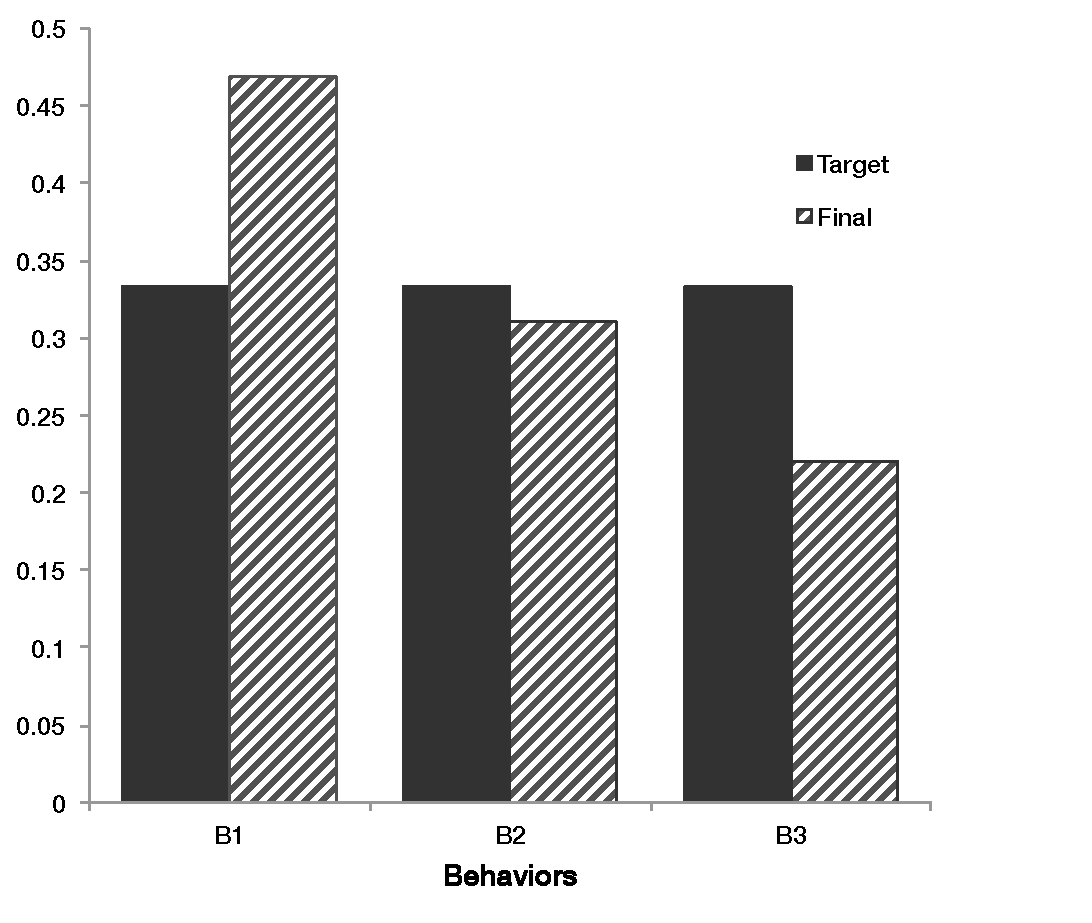
\includegraphics[width=\columnwidth]{coll-dist}
\par\end{centering}
\caption{A comparison of the final equilibrium distribution and the desired target $q$ of uniform distribution of behaviors when the seed distribution $p_{seeds}$ is set to be uniform. The results are for the collaboration network (COLL). Low cost behaviors spread more than do high-cost behaviors. The KL divergence between the equilibrium behavior distribution and the target $q$ is 0.05.}\label{fig:snap-uniform}
\end{figure}

Figure~\ref{fig:comparison} shows the comparison in resource utilization with different values of $\alpha$ the fraction of seeds in the network. We show four seed selection heuristics: random, na\"ive with resource top up, degree and resource ranked seeds and the expected immediate maximization heuristic with hill climbing (H7). In this simulation the behaviors were distributed uniformly across all the seeds. The heuristic H7 consistently outperforms the other three seed selection heuristics, for each value of $\alpha$.  

\begin{figure}[htb]
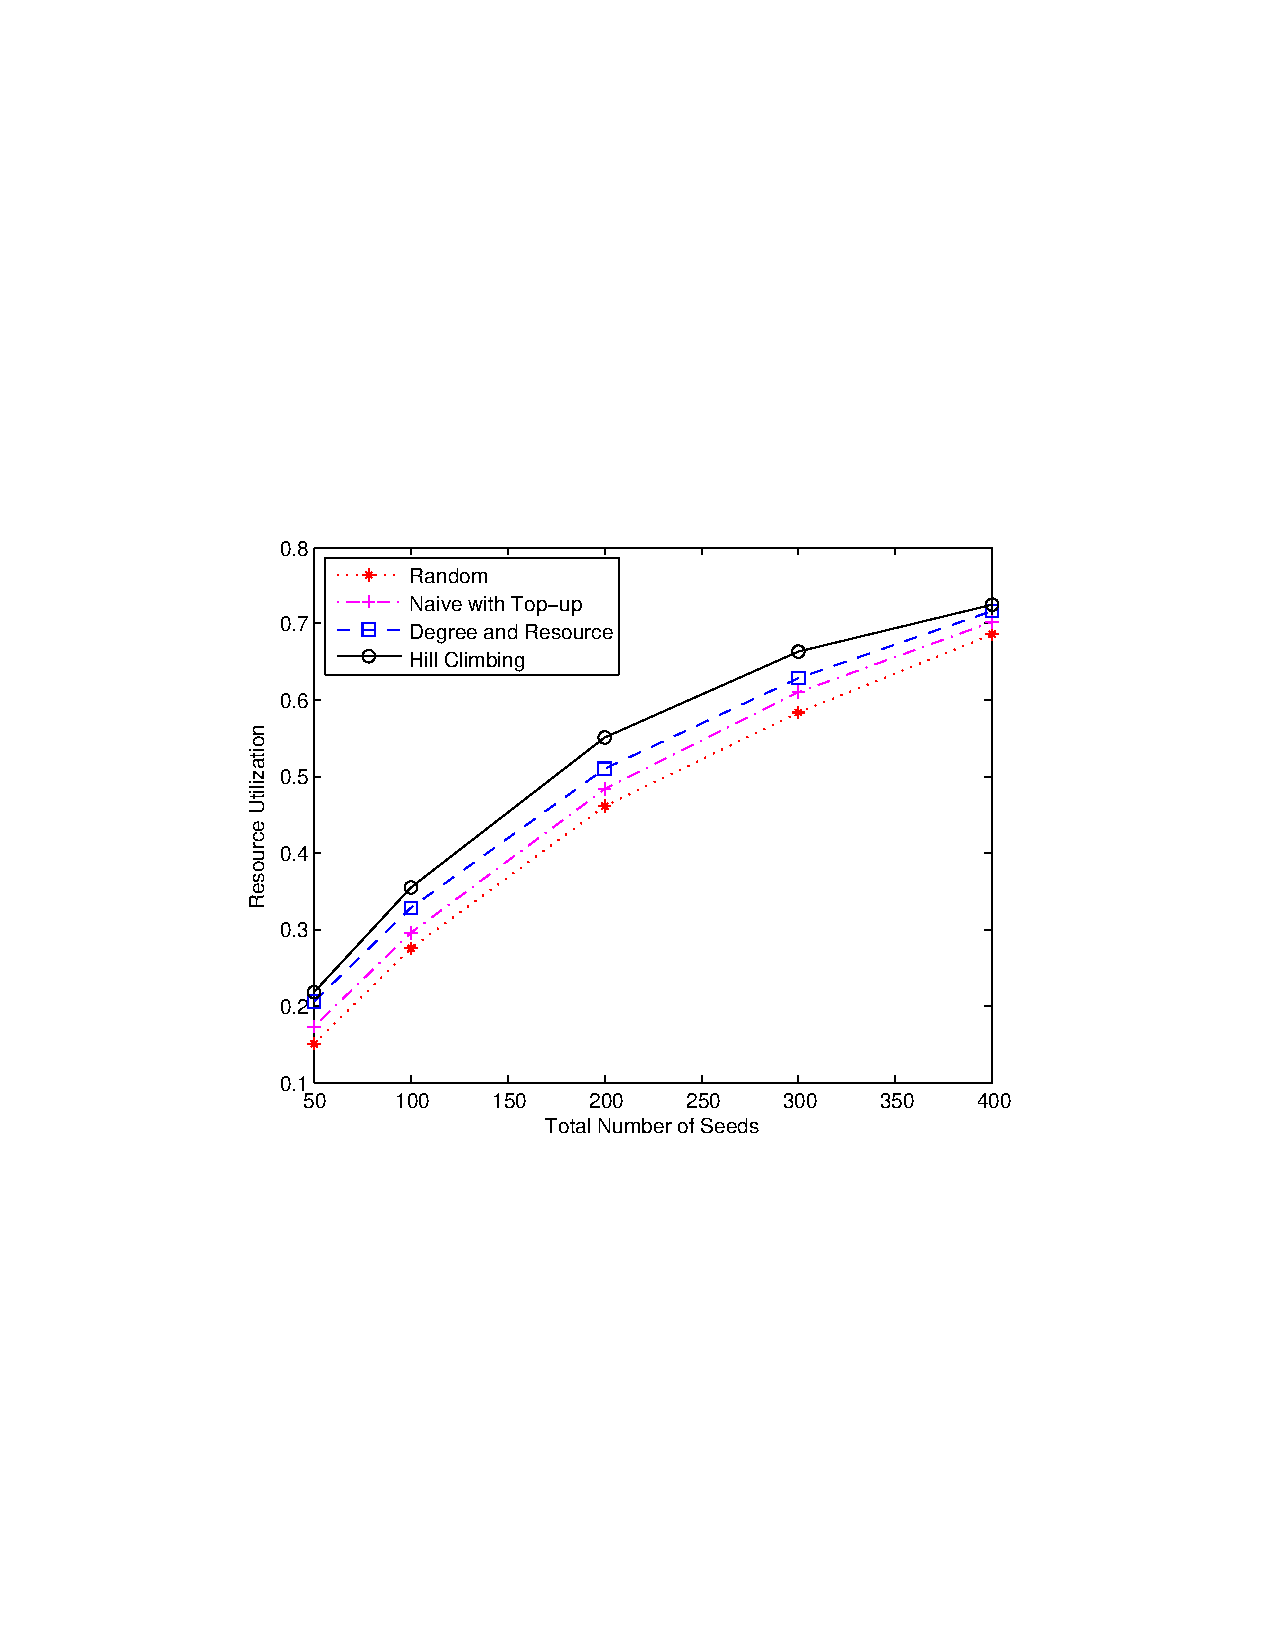
\includegraphics[viewport=1.5in 3.5in 6.75in 7.5in, width=\columnwidth]{comp}
\caption{The graph shows the comparison in resource utilization with the different number of seeds (that is, different values of the $\alpha$ parameter, for four heuristics. The heuristic H7, which maximizes Influence Weight  performs the best. Notice that $l=50$ corresponds to $\alpha=0.1$.}\label{fig:comparison}
\end{figure}

\section{Discussion and Open Issues}\label{sec:disc}
One of the main motivations of the present work was to develop a realistic model of the behavior diffusion process. There are many ways in which our work can be extended. Here we discuss about a few such possible extensions.
    
Our present model does not consider the role of behavioral inertia in the diffusion process. Often people are hesitant of adopting new behaviors because they cannot free their resources from practicing an old behavior which possibly has less value. This can be modeled in our framework by introducing an additional benefit for the already adopted behaviors. Another technique would be to introduce epidemic models such as SIRS to better model long-term behavioral adoption. 

In a network, we receive social signals from our friends, but there is noise because we miss messages and or we check them late. In modeling the behavior adoption problem, we have ignored the role of constraints in how they affect the production and consumption of messages from peers. Explicit consideration of the cost of social signaling would not only make the model more realistic and provide better bounds on the maximal resource utilization of the networks resources.

\section{Conclusions}\label{sec:conclusion}
In this paper we have considered the problem of seed selection to maximize resource utilization and to achieve a specified target distribution for multiple behavior diffusion processes.  We are motivated by collective action problems with applications to sustainability and public health. We have considered a social network where individuals are constrained by available resources for adoption of new behaviors. Our work is the first of its kind, to the best of our knowledge to study the influence of individual resource constraints on multiple, costly behavior adoption. Mindful of the confound between homophily and structural effects, individuals in our model respond to the social influence as well as the intrinsic utility of a spreading behavior. We have shown that the core optimization problems are NP-complete and provided novel heuristics for solving them. We have tested our heuristics against the random and na\"ive methods and have shown that our heuristics perform very well. We have also shown that assigning the target distribution as the behavior distribution over the seed set results in the final diffused behaviors being very close to the target distribution. Some of the open issues include the use of epidemic models for modeling long-term behavior adoption and incorporating the idea of noisy social signals in modeling behavior adoption.


% Appendix
\appendix
\section*{APPENDIX}
%\setcounter{section}{1}
\section{Computation of Immediate Adoption Probability}
\label{sec:ia-comp}
In this section we discuss an example of how the different immediate behavior adoption probabilities for a node are computed. This computation depends on whether all the thresholds of a node have the same random value (\emph{matched threshold}) or independent and uniformly distributed random values (\emph{different threshold}). Although all the results in this paper are for the \emph{different threhsold} model, her we present examples for both cases for the sake of completeness. Suppose a vertex $v$ has $8$ neighbors. According to our threshold model each of its neighbors exerts an influence of $0.125$ on it. Suppose $v$ is already a seed for behavior \emph{A}; moreover it has $2$ neighbors with behaviors \emph{B}, and $3$ neighbors with behavior \emph{C}. We are interested in computing the probabilities that it will adopt each of the three behaviors in the next time step. 

\subsection{Matched Threshold:}
In this case, for any vertex the thresholds for all the three behaviors will be the same, but it will be assigned independently of other nodes and uniformly at random from the interval $[0,1]$. So if $v$'s threshold is in the interval $[0,0.25]$, then $v$ will consider both behaviors B and C together with A for adoption. Our payoff maximizing behavior adoption process dictates that it will adopt a subset of \emph{A,B} and \emph{C} that will provide maximum combined payoff subject to the resource constraint of the node. This adoption decision process is equivalent to solving a knapsack problem. We will solve the knapsack problem and decide which behaviors out of the three behaviors - A, B and C - will be adopted. Any such behavior will be adopted with probability $0.25.$ 

If $v$'s threshold is in the interval $(0.25,0.375]$ then $v$ will only consider behavior C together with behavior A for adoption. Again after solving knapsack problem and deciding which behaviors to adopt out of A and C, it will adopt any such behavior with probability $0.125$. 

At last if $v$'s threshold is in the interval $(0.375,1]$ then it will definitely adopt behavior A - the probability of which is $1-0.375=0.625$. In the worst case the complexity of this probability computation process for each node is linear order of the number of behaviors.

\subsection{Different Threshold:}
In the \emph{different threshold} case, for each vertex the thresholds are assigned independently and uniformly at random from the interval $[0,1]$. So in this case we need to consider all possible combinations of behaviors B and C together with A (which will always be considered) and work out the individual probabilities. The worst case computational complexity of this process for each node will be exponential in the number of behaviors. In our example we need to consider the following cases:
\begin{enumerate}
\item[i)] B and C together with A; any behavior selected by the knapsack algorithm will be adopted with probability $0.25\times0.375=0.09375$.
\item[ii)] B together with A; any behavior selected by the knapsack algorithm will be adopted with probability $0.25\times(1-0.375)=0.15625$.
\item[iii)] C together with A; any behavior selected by the knapsack algorithm will be adopted with probability $(1-0.25)\times0.375=0.28125$.
\item[iv)] Only A; A will be adopted with probability $(1-0.25)\times(1-0.375)=0.46875$.
\end{enumerate}

\section{Variants of Seed Selection Algorithm} \label{sec:t-nt-comp}
Table \ref{tab:t-nt-comp} presents the Total Participation and Total Adoption values for the different variants of the KKT seed selection algorithm and IA based seed selection heuristic. T versions provide better spread than the NT versions which is expected since more resource is required for starting the diffusion in the T version. However for the same type of top up regime there is not much difference between the S and M version. If we consider exact algorithms instead of heuristics and approximation algorithms, then it is easy to see that S version can never produce a result that is better than the M version, since solution for S version is also a valid solution for M version. This fact accounts for the absence of any real difference between the S and T versions in the case of the heuristic and the approximate algorithm. 
\begin{table}[htb]\footnotesize
    \centering
    \caption{Total Participation / Total Adoption under different networks as \% of the network size. S and M variants give almost identical results with T variants exceeding NT variants.}\label{tab:t-nt-comp}
    \begin{tabular}{cccc} \toprule
        Heuristics & PA & SW & SC \\ \midrule
        KKT-S-T & 43.7 / 44.5 & 26.2 / 26.4 & 27.3 / 27.3  \\
        H8-S-T & 43.9 / 44.5 & 23.6 / 24.5 & 23.6 / 24.2 \\ 
        \midrule
        KKT-S-NT & 39.5 / 39.5 & 21.7 / 22.0 & 22.0 / 22.5  \\
        H8-S-NT & 39.51 / 39.8 & 22.7 / 23.2 & 20.0 / 20.5 \\ 
        \midrule
        KKT-M-T & 43.7 / 44.5 & 26.2 / 26.4 & 27.1 / 27.1  \\
        H8-M-T & 39.0 / 45.8 & 22.8 / 23.5 & 21.9 / 22.6 \\ 
        \midrule
        KKT-M-NT & 39.5 / 39.5 & 21.7 / 22.0 & 22.4 / 23.0  \\
        H8-M-NT & 39.5 / 43.3 & 22.7 / 23.2 & 19.7 / 21.1 \\ 
        \bottomrule
        
    \end{tabular}
\end{table}

%\appendixhead{ZHOU}

% Acknowledgments
\begin{acks}
%The authors would like to thank Dr. Maura Turolla of Telecom
%Italia for providing specifications about the application scenario.
\end{acks}

% Bibliography
\bibliographystyle{ACM-Reference-Format-Journals}
\bibliography{refs}

% History dates
%\received{February 2007}{March 2009}{June 2009}

% Electronic Appendix
\elecappendix

\medskip

%\section{This is an example of Appendix section head}
%Channel-switching time is measured as the time length it takes for


%\section{Appendix section head}
%The primary consumer of energy in WSNs is idle listening. The key to

\end{document}



